\documentclass[12pt]{article}

\usepackage[utf8]{inputenc}
\usepackage{amsmath}
\usepackage{graphicx}
\usepackage{geometry}
\geometry{a4paper, margin=1in}
\usepackage{hyperref}
\newcommand{\note}[1]{\textbf{#1}} % Makes the term bold

\begin{document}

\begin{titlepage}
    \centering

    \vspace*{1cm}

    \rule{\textwidth}{1pt}

    \vspace{2\baselineskip}

    {\huge  Cyber Security } \\

    \vspace{1\baselineskip}

    {\huge \textbf{ Lab 1 - Web Application Vulnerabilities }}

    \vspace{2\baselineskip}

    \rule{\textwidth}{1pt}

    \vspace{1cm}

    \large

    \begin{flushleft}
        \begin{minipage}{.8\textwidth}
            \raggedright
            Fullname: Amangeldi Zhanserik \\
            ID: 22B030301 \\
            E-mail: {\normalsize \url{zha_amangeldi@kbtu.kz}} \\
            Date of submission: \today \\
            Class time: Thursday, 15:00--18:00 \\
        \end{minipage}%
    \end{flushleft}

    \vspace{2cm}

    
\includegraphics[width=.7\textwidth]{logo-kbtu.png}

    \vfill

    School of Information System and Engineering \\
    Kazakh-British Technical University \\
    Academic Year 2024-2025 \\
\end{titlepage}

\section{Introduction}

This lab aims to provide hands-on experience with common web application vulnerabilities. We will be using two resources: Hacksplaining for interactive security training and OWASP Top 10 for understanding industry-standard security practices.

\section{Part 1: Hacksplaining Security Training for Developers}

\subsection{Sign Up for Hacksplaining}

\begin{enumerate}
    \item Go to \url{https://www.hacksplaining.com/}. \\
    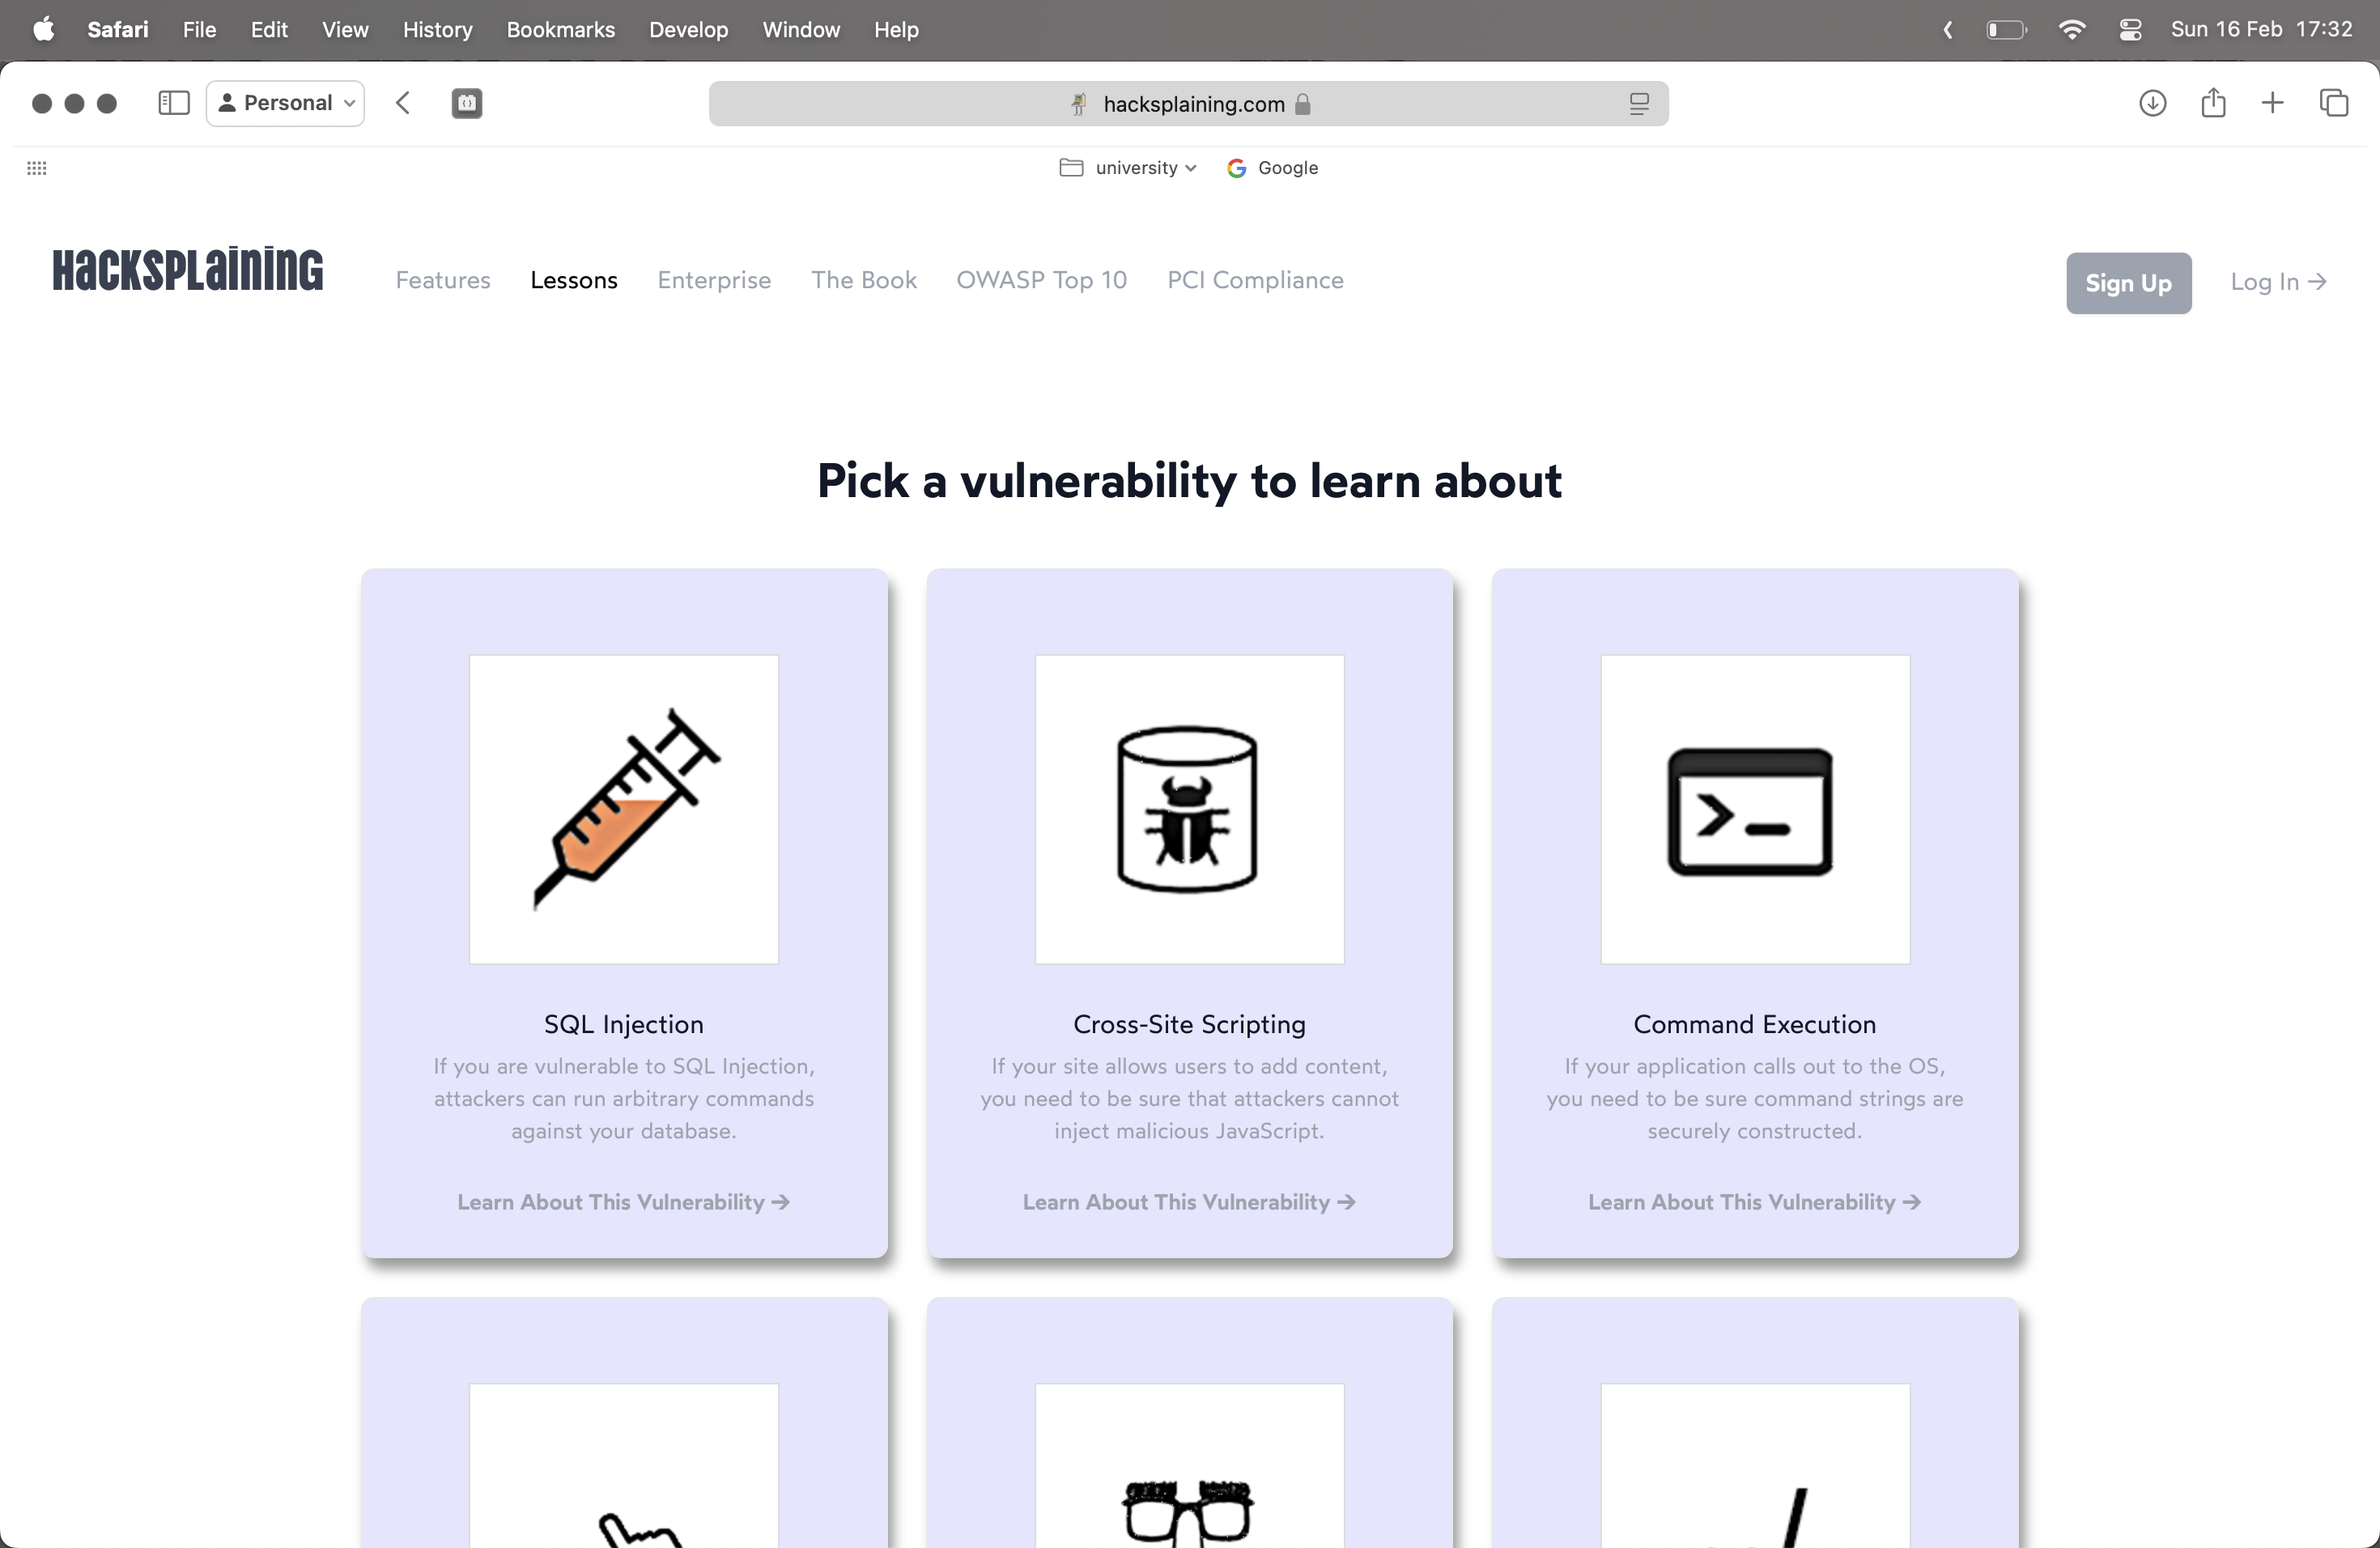
\includegraphics[width=0.5\textwidth]{Image1.png}
    \item Click on "Sign Up". \\
    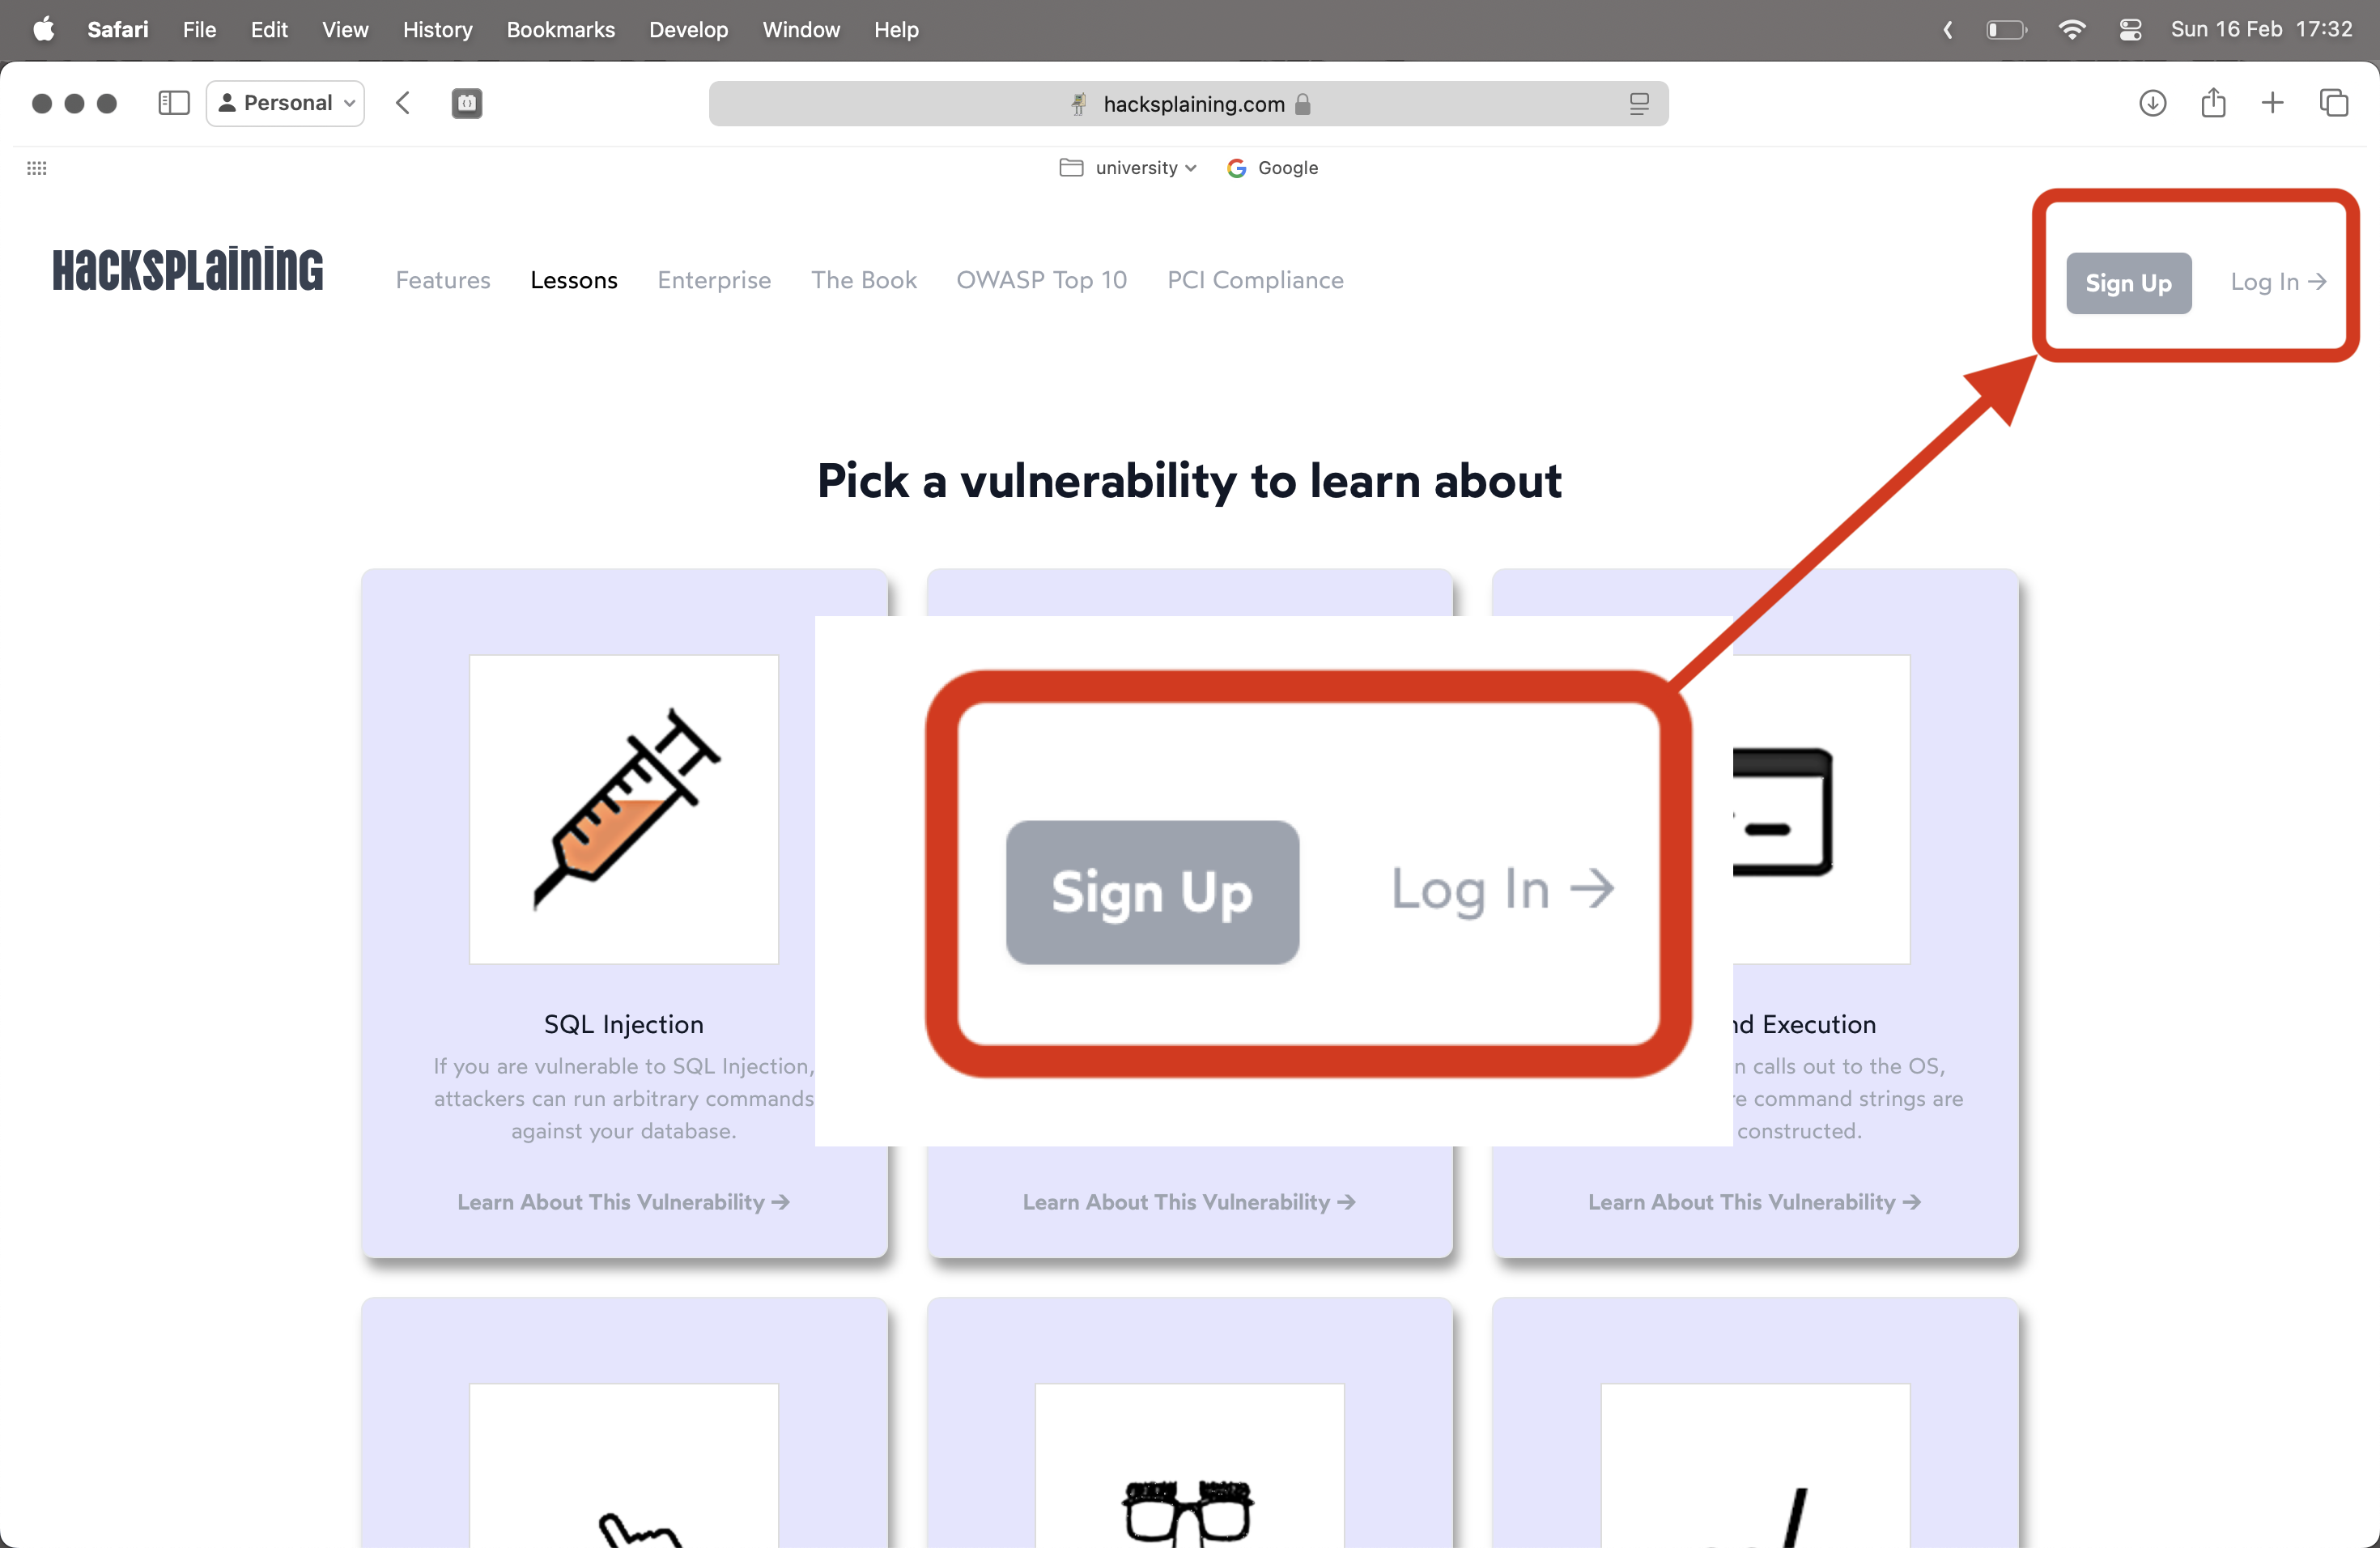
\includegraphics[width=0.5\textwidth]{Image2.png}
    \newpage
    \item Choose your own way to register(Email, Github or Google). I chose Google. \\
    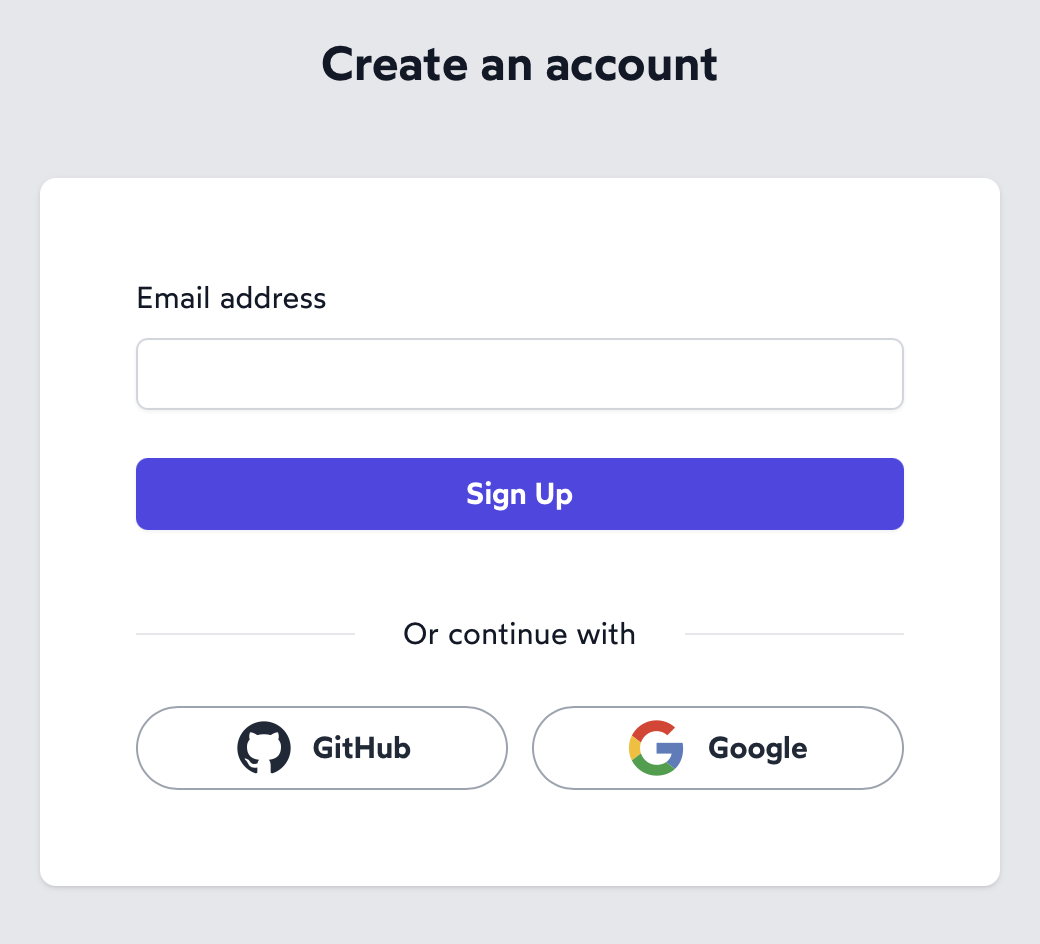
\includegraphics[width=0.5\textwidth]{Image3.png}
\end{enumerate}

\subsection{Explore Web Application Vulnerabilities}

Once logged in, I explored the following vulnerabilities:

\begin{itemize}
    \item Clickjacking
    \item Cross-Site Request Forgery
    \item Cross-Site Scripting
    \item SQL Injection
    \item Directory Traversal
    \item Command Execution
    \item Denial of Service Attacks
\end{itemize}

\newpage

\subsubsection{Clickjacking}
Clickjacking is a malicious technique to trick a user into clicking on something different from what the user perceives they are clicking on. Clickjacking has been used to: \\
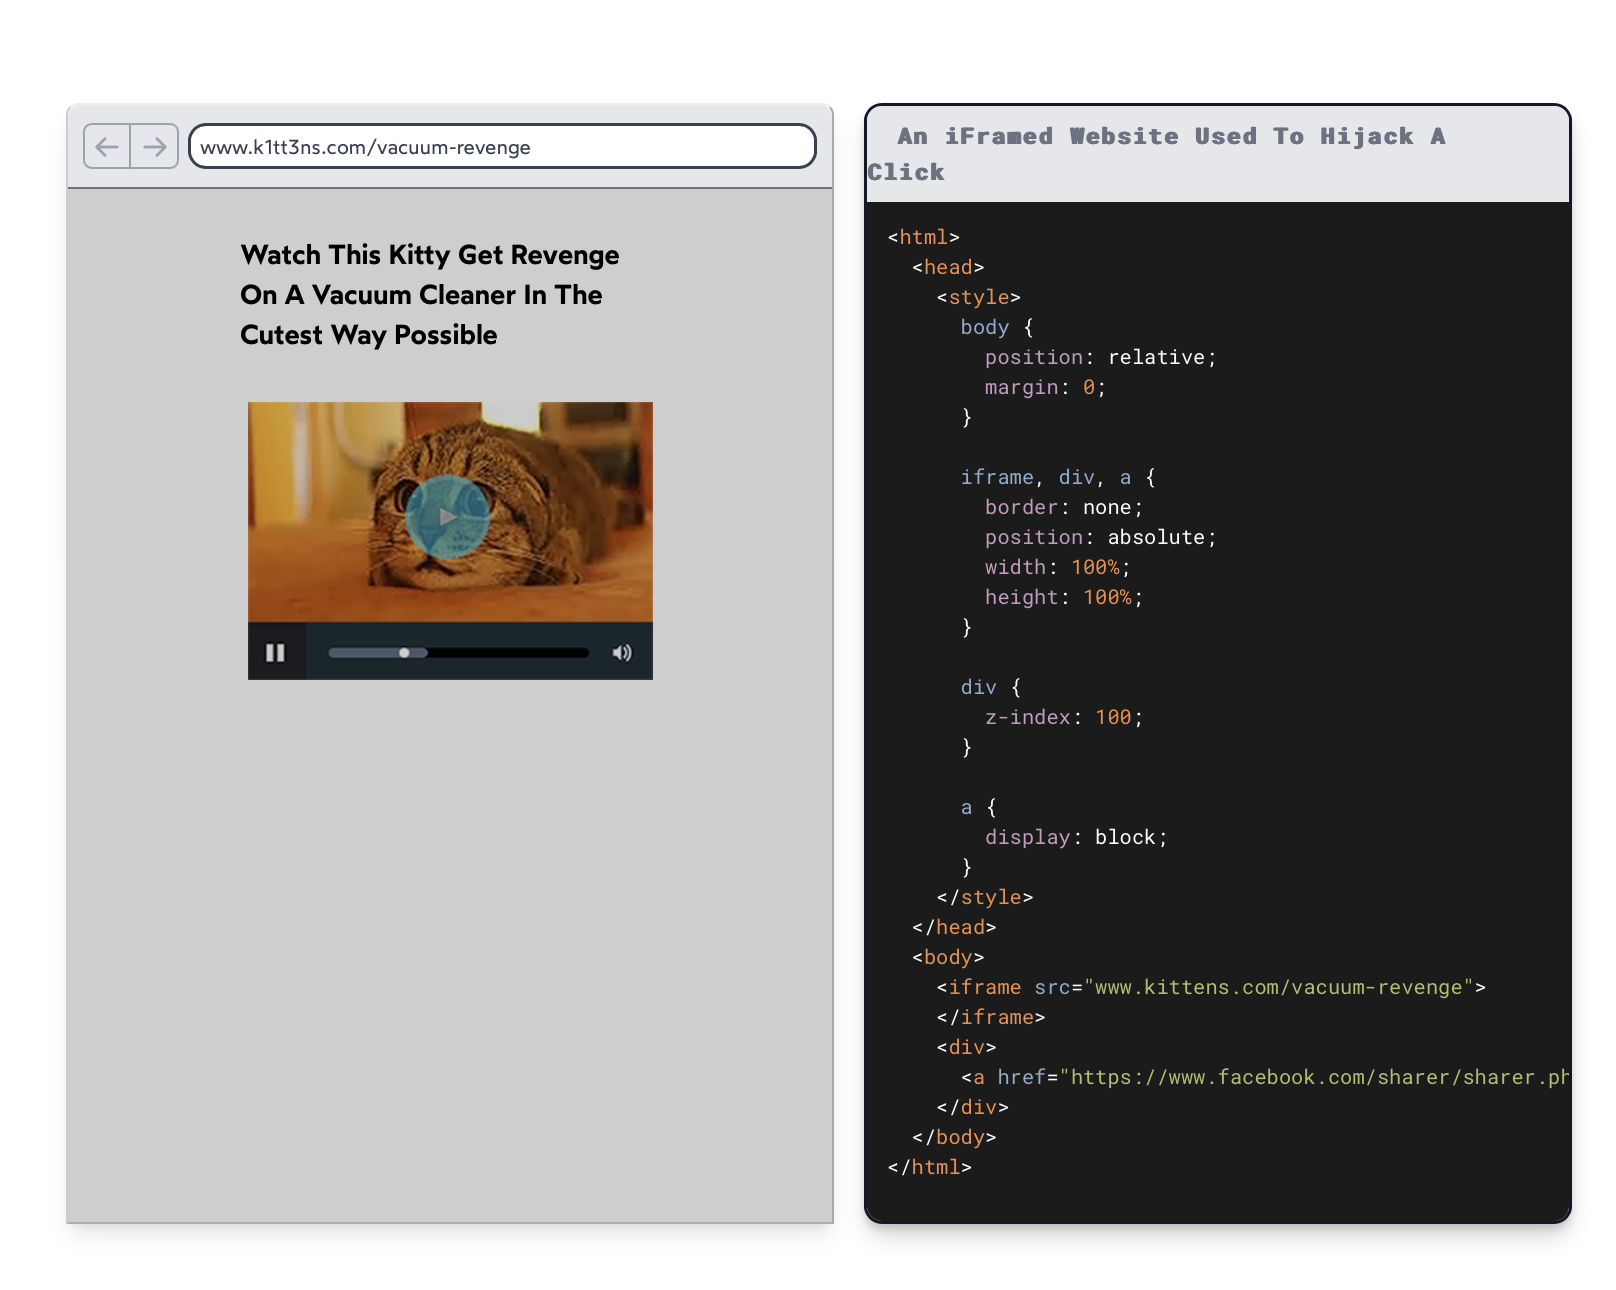
\includegraphics[width=.7\textwidth]{Image15.png} 
\begin{itemize}
    \item Harvest login credentials
    \item Trick users into turning on their web-cam or microphone
    \item Spread worms on social media sites
    \item Promote online scams
    \item Spread malware
\end{itemize}
There are several ways to protect from Clickjacking:
\begin{itemize}
    \item Content Security Policy (CSP)
    \item X-Frame-Options
    \item Frame-Killing Code
\end{itemize}
\note{Note}: Clickjacking won't affect your site directly, but it could potentially affect your users. And only you can protect them! \\

\newpage

\subsubsection{Cross-Site Request Forgery}
Cross-Site Request Forgery (CSRF) is an attack that forces an end user to execute unwanted actions on a web application in which they are currently authenticated. CSRF attacks have been used to: \\
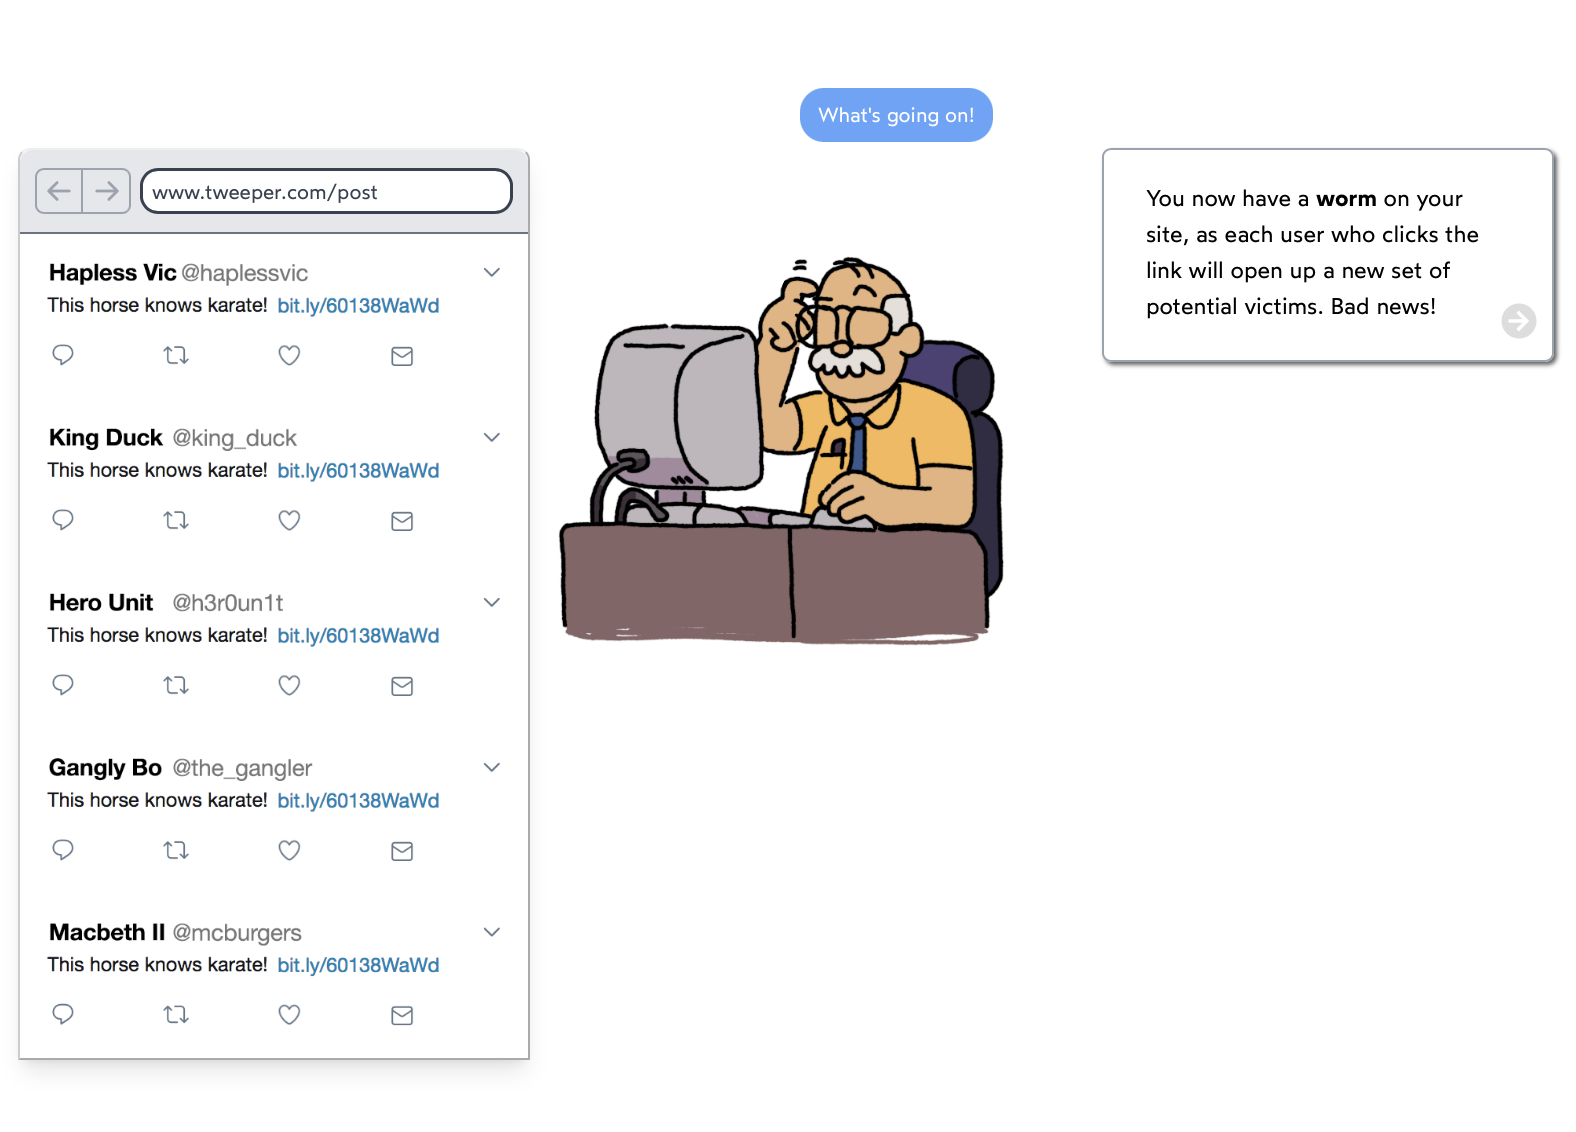
\includegraphics[width=.7\textwidth]{Image16.png}
\begin{itemize}
    \item Steal Confidential Information.
    \item Spread warms on social media.
    \item Install malware on mobile phones
\end{itemize}
There are several ways to protect from CSRF:

\begin{itemize}
    \item Anti-CSRF Tokens.
    \item SameSite Cookie Attribute.
    \item Include Addition Authentication for Sensitive Actions.
    \item Representation State Transfer (REST) APIs.
\end{itemize}
\note{Note}: CSRF attacks can be very damaging, especially if the victim is an administrative user. Therefore, it is crucial to implement proper CSRF protection mechanisms.

\newpage

\subsubsection{Cross-Site Scripting}
Cross-Site Scripting (XSS) is a security vulnerability that allows an attacker to inject malicious scripts into web pages viewed by other users. XSS attacks have been used to:
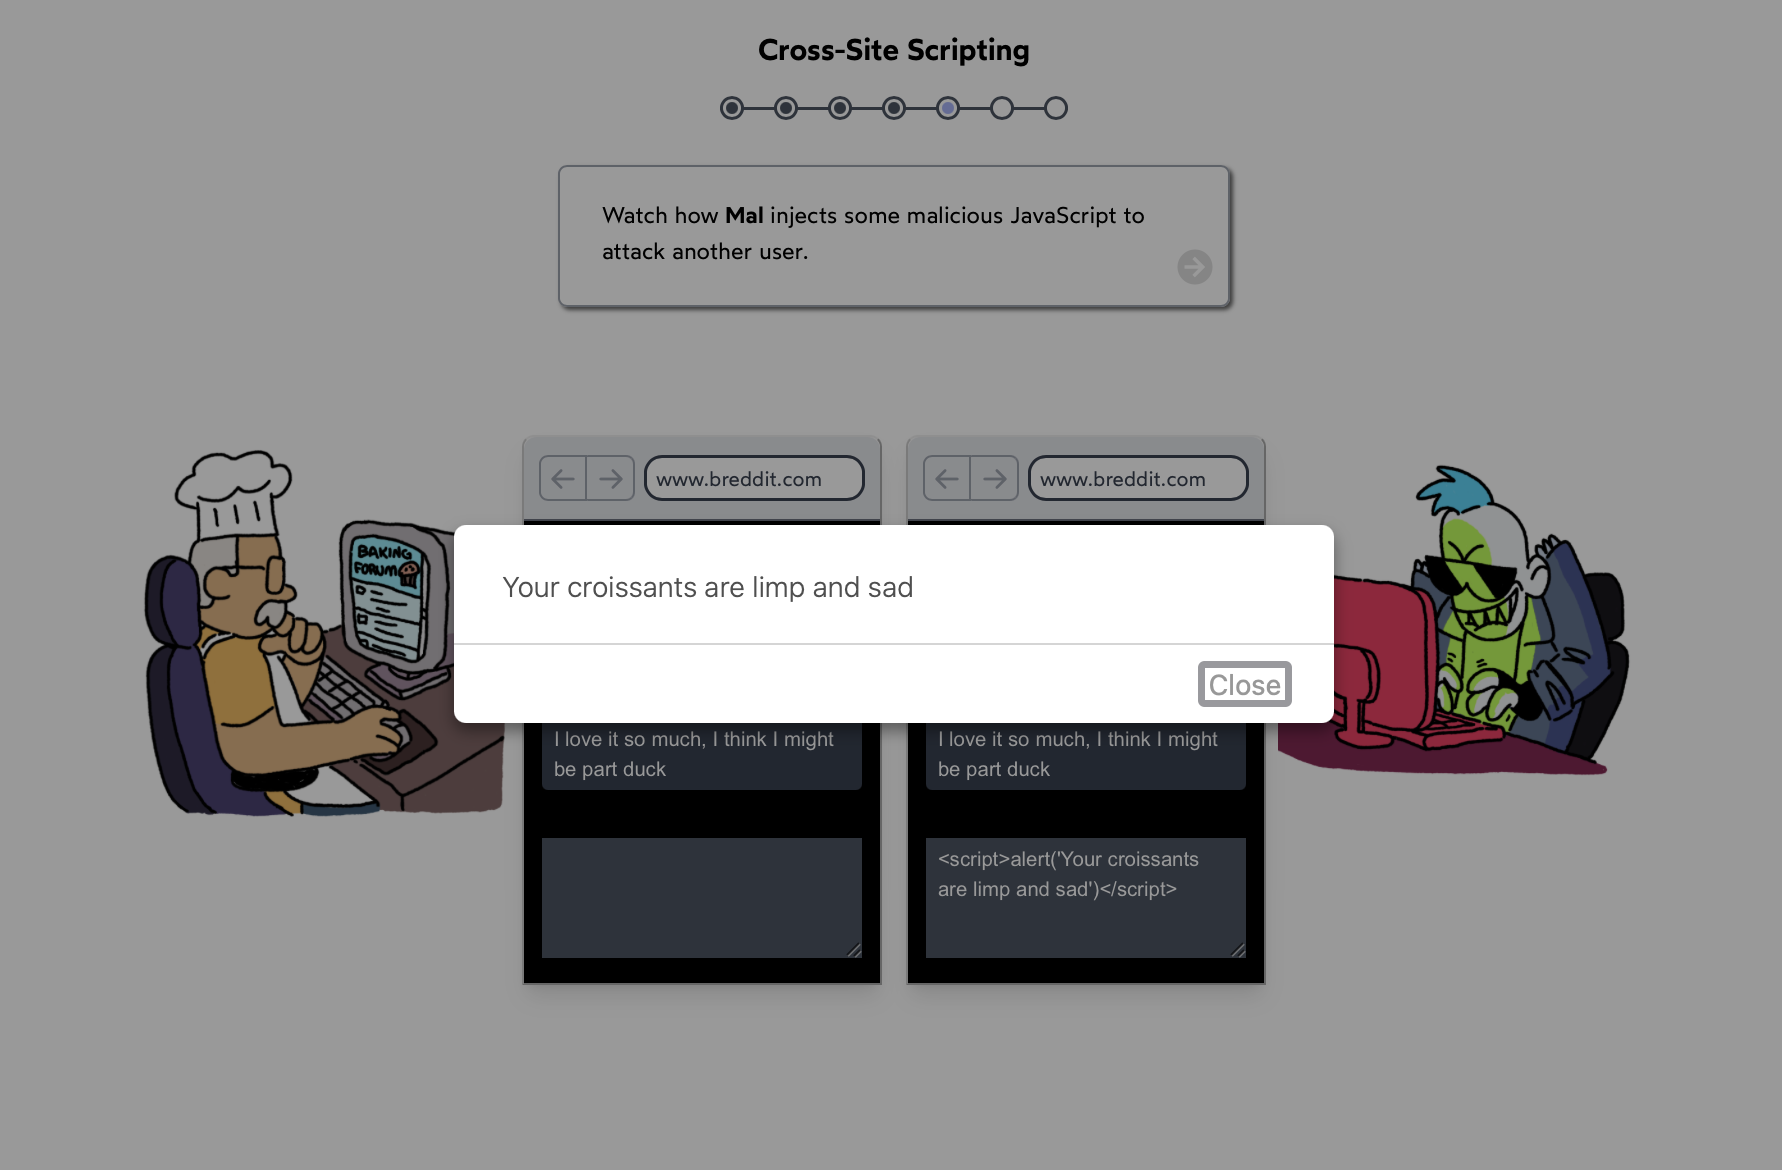
\includegraphics[width=.7\textwidth]{Image17.png}
\begin{itemize}
    \item Spreading worms on social media.
    \item Session Hijacking.
    \item Identity Theft.
    \item Denial of service attacks and website vandalism.
    \item Theft of sensitive data.
    \item Financial fraud.
\end{itemize}
There are several ways to protect from XSS:

\begin{itemize}
    \item Escape dynamic content.
    \item Allowlist Values.
    \item Implement a Content Security Policy (CSP).
    \item Sanitize HTML
\end{itemize}
\note{Note}: Avoid reading or manipulating cookies in client-side JavaScript. Mark cookies as HTTP-only to ensure they are handled by the browser and not accessible via JavaScript.

\newpage

\subsubsection{SQL Injection}
SQL Injection is a code injection technique that might destroy your database. SQL Injection attacks have been used to: \\
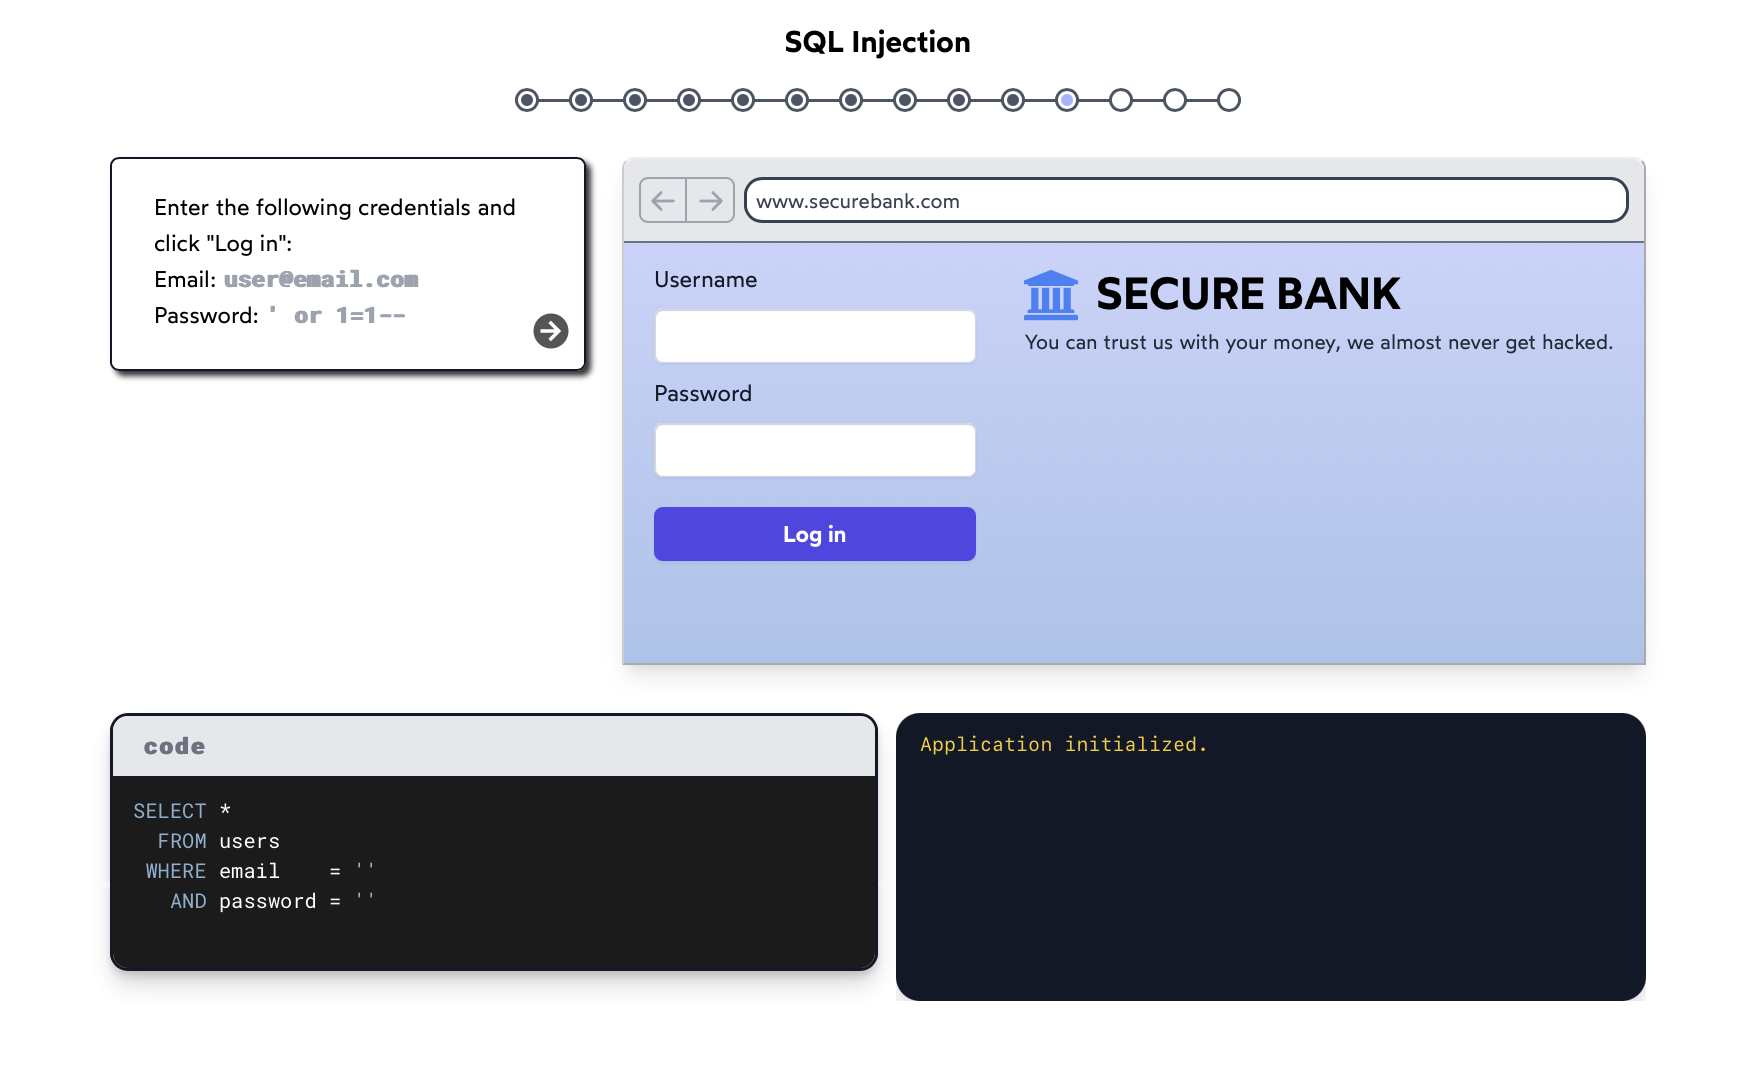
\includegraphics[width=.7\textwidth]{Image18.png}
\begin{itemize}
    \item Extract sensitive information.
    \item Enumerate the authentication details of users registered on a website.
    \item Delete data or drop tables.
    \item Inject further malicious code.
\end{itemize}
Simple example of SQL Injection: \\
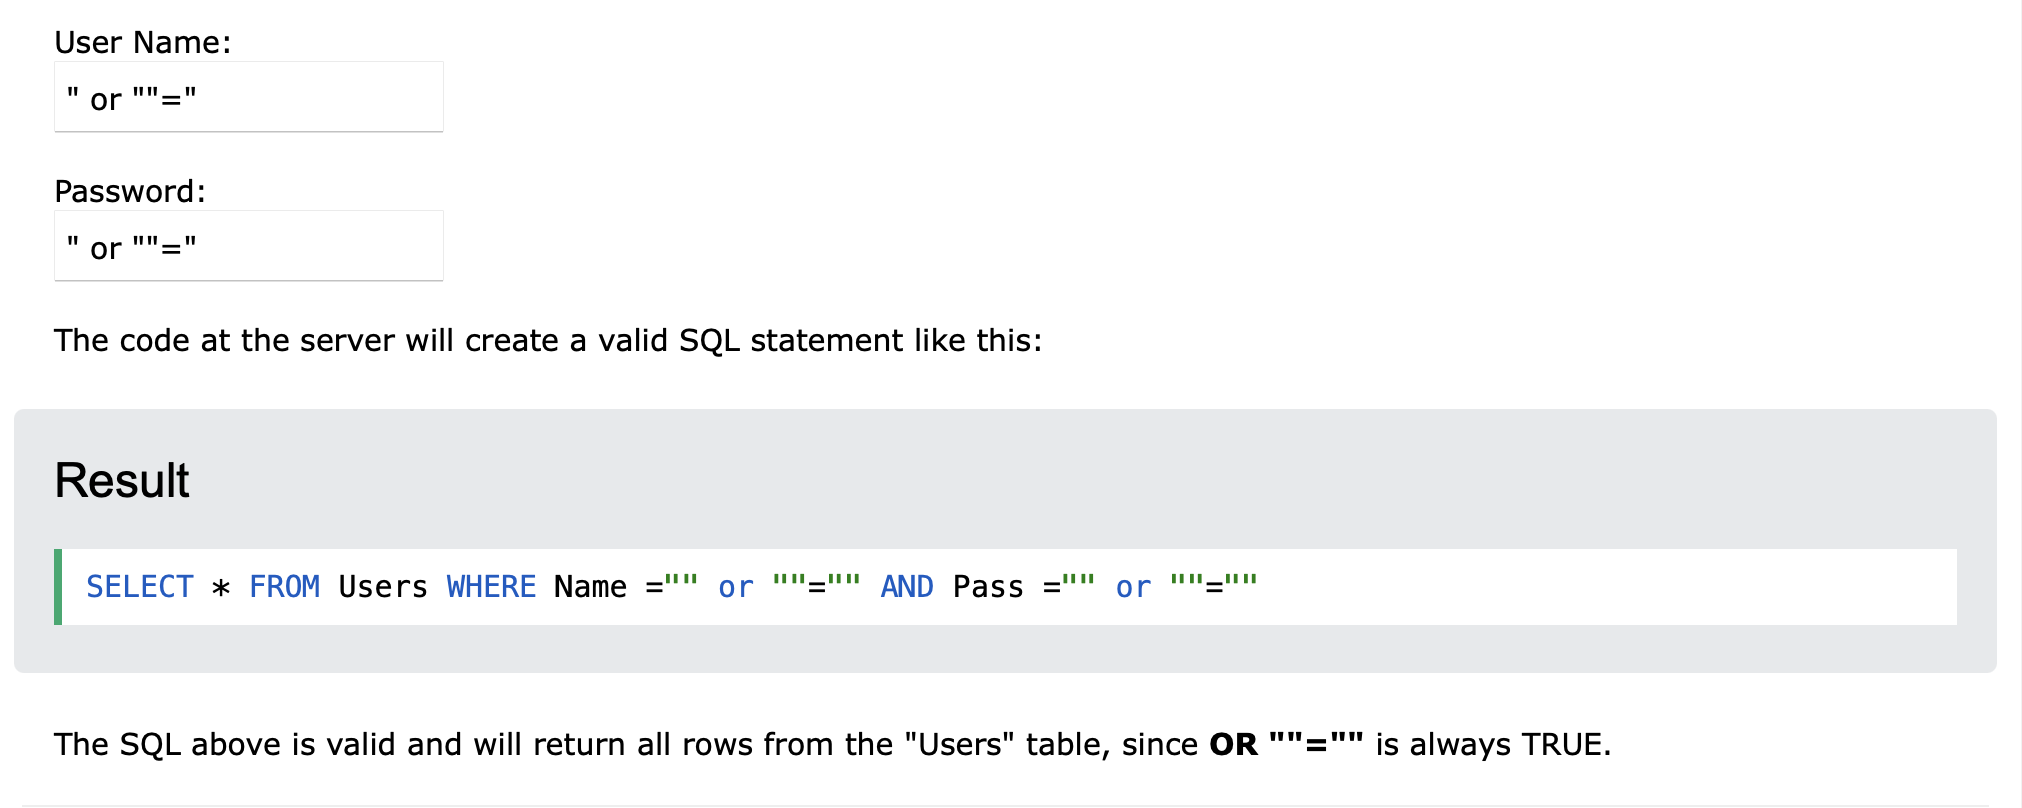
\includegraphics[width=1\textwidth]{Image4.png}
Protection from SQL Injection:
\begin{itemize}
    \item Parameterized Queries.
    \item Using Object Relational Mapping (ORM).
    \item Escaping some symbol characters.
    \item Sanitize user input.
\end{itemize}

\newpage

\subsubsection{Directory Traversal}
Directory traversal vulnerabilities allow attackers to access arbitrary files on your system by manipulating URL paths. If an attacker discovers a directory traversal vulnerability, they can access sensitive files, such as configuration files, source code, and more. Protection from Directory Traversal: \\
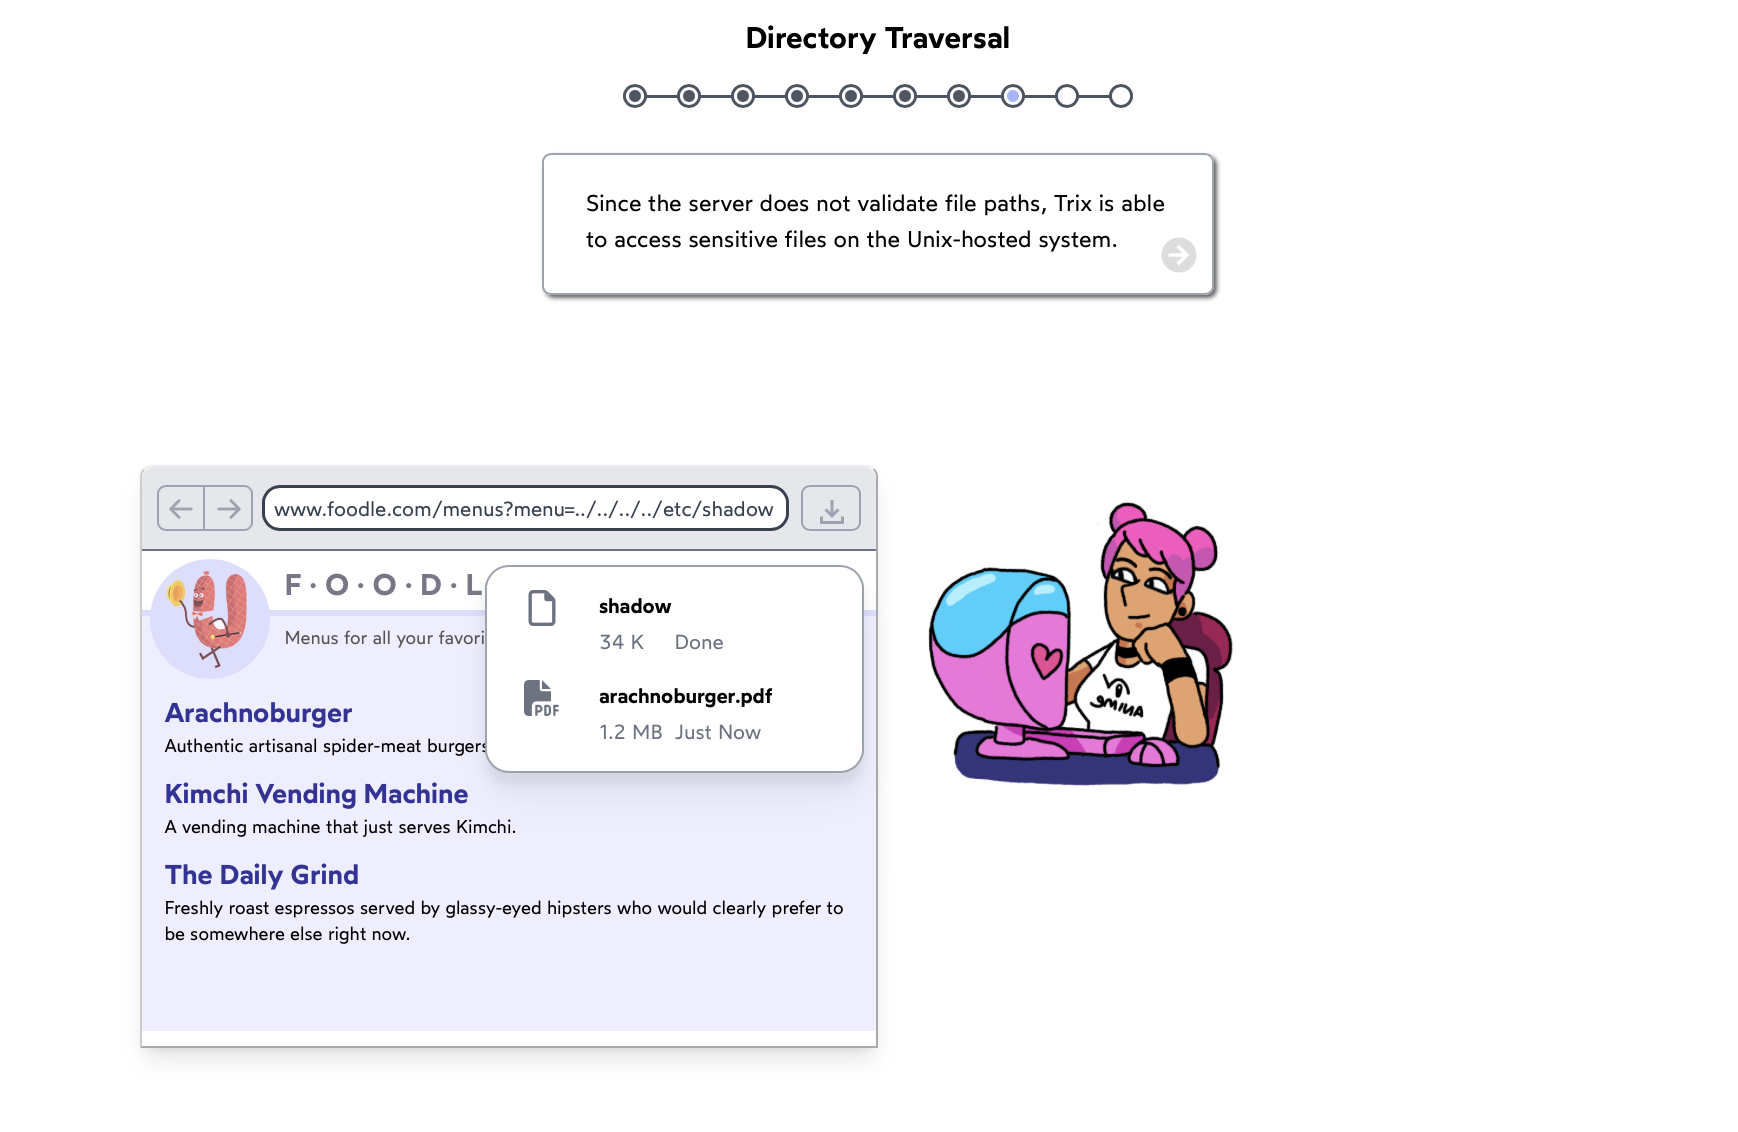
\includegraphics[width=.7\textwidth]{Image19.png}
\begin{itemize}
    \item Use a content management system (CMS) that has built-in security features.
    \item Use Indirection. Each time a file is uploaded, construct a "friendly" name for this on your site, and when the file is accessed, perform a lookup in your data-store to discover the actual file path.
    \item Segregate Your Documents
    \item Sanitize Filename Parameters. The safest approach is to restrict filenames to a list of known good characters, and ensure that any references to files use only those characters.
    \item Run server processes with Restricted Permissions.
\end{itemize}

\newpage

\subsubsection{Command Execution}
Command Execution is a major security lapse that allows an attacker to execute arbitrary commands on your server. Protection ways: \\
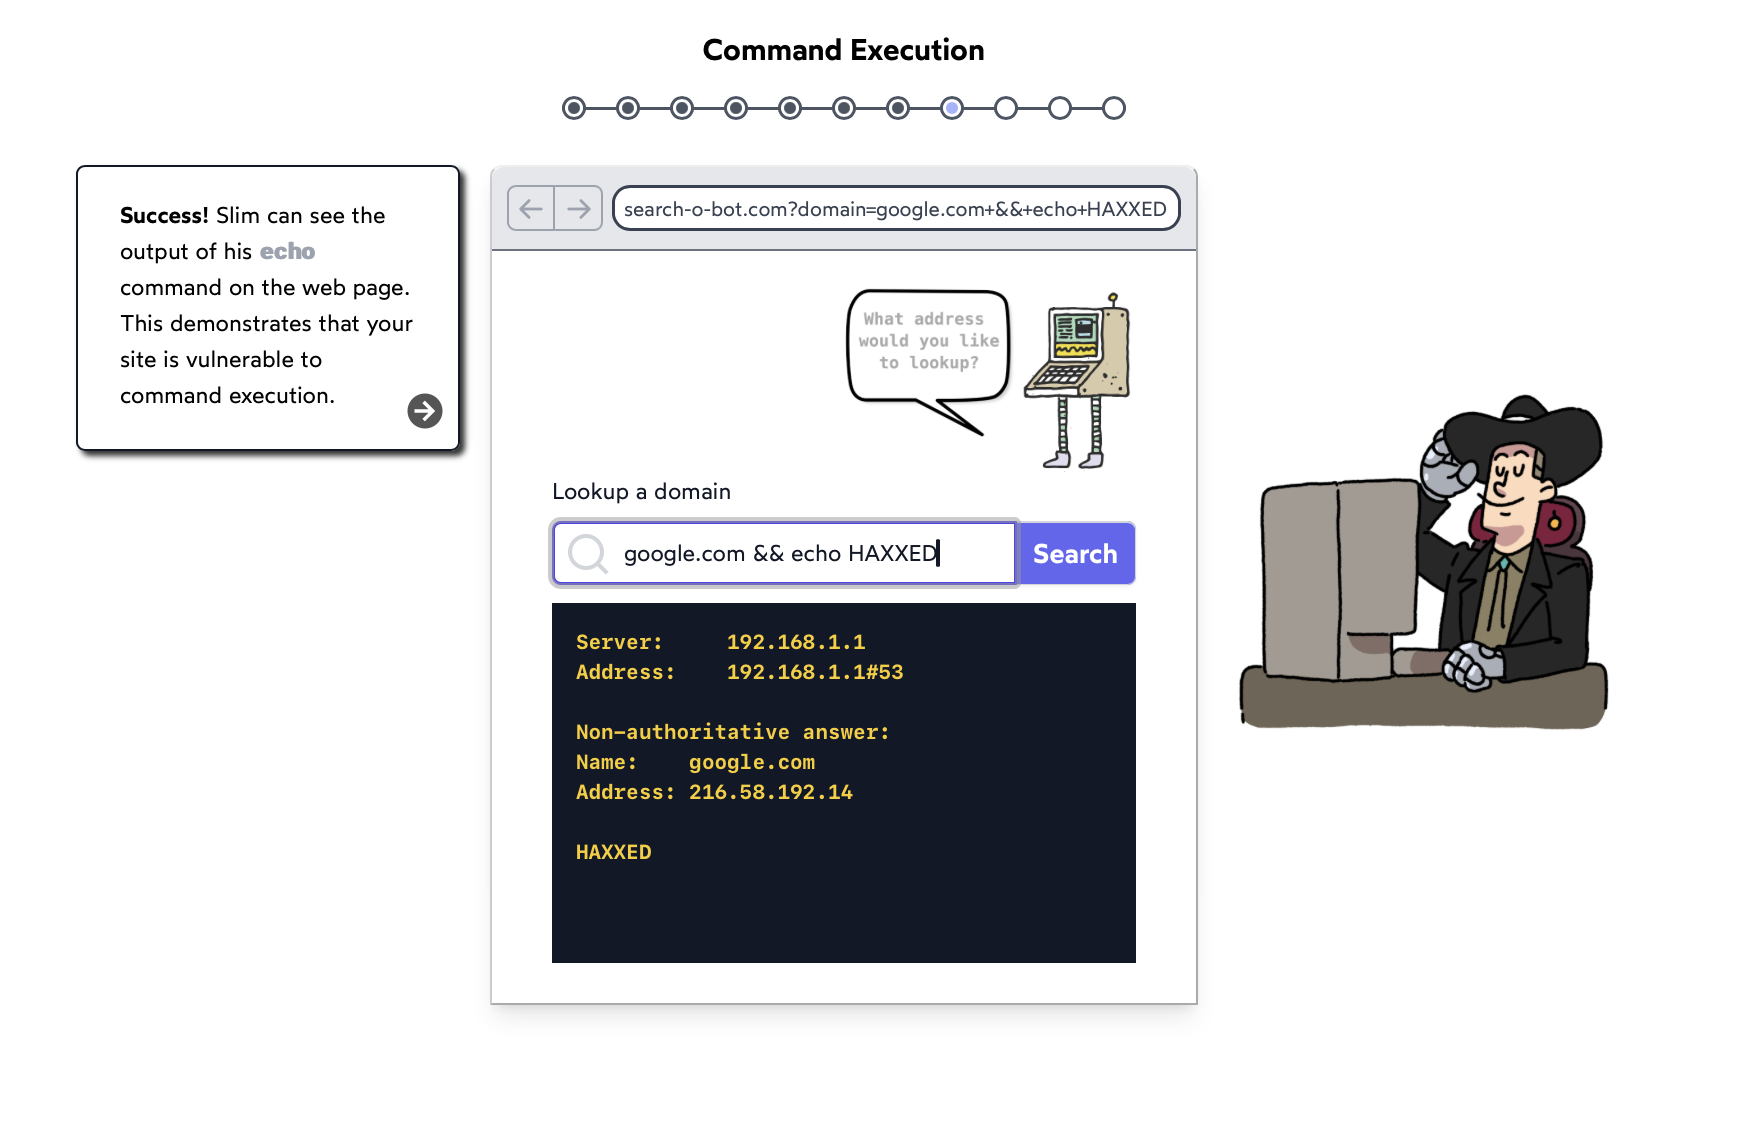
\includegraphics[width=.7\textwidth]{Image20.png} 
\begin{itemize}
    \item Try to Avoid Command Line Calls Altogether. Use APIs whenever possible.
    \item Escape Inputs Correctly
    \item Restrict the Permitted Commands
    \item Perform Thorough Code Reviews
    \item Run server processes with Restricted Permissions
\end{itemize}

\subsubsection{Denial of Service Attacks}
Denial-of-service attacks aim to make a site unavailable to users. They can be politically motivated, for extortion, or to cause disruption. Attackers often use distributed applications to flood a site from multiple IP addresses, making it hard to filter out all sources. 

To protect against denial-of-service attacks, consider using commercial tools and services. Many cloud providers offer basic protection and alerting for free, with advanced options available at additional cost.

\newpage

\section{Part 2: Understanding OWASP Top 10}

\subsection{Open OWASP Top 10}

I visited \href{https://hacksplaining.com/owasp}{the OWASP Top 10 webpage} to explore the top 10 web application security risks. \\ \\
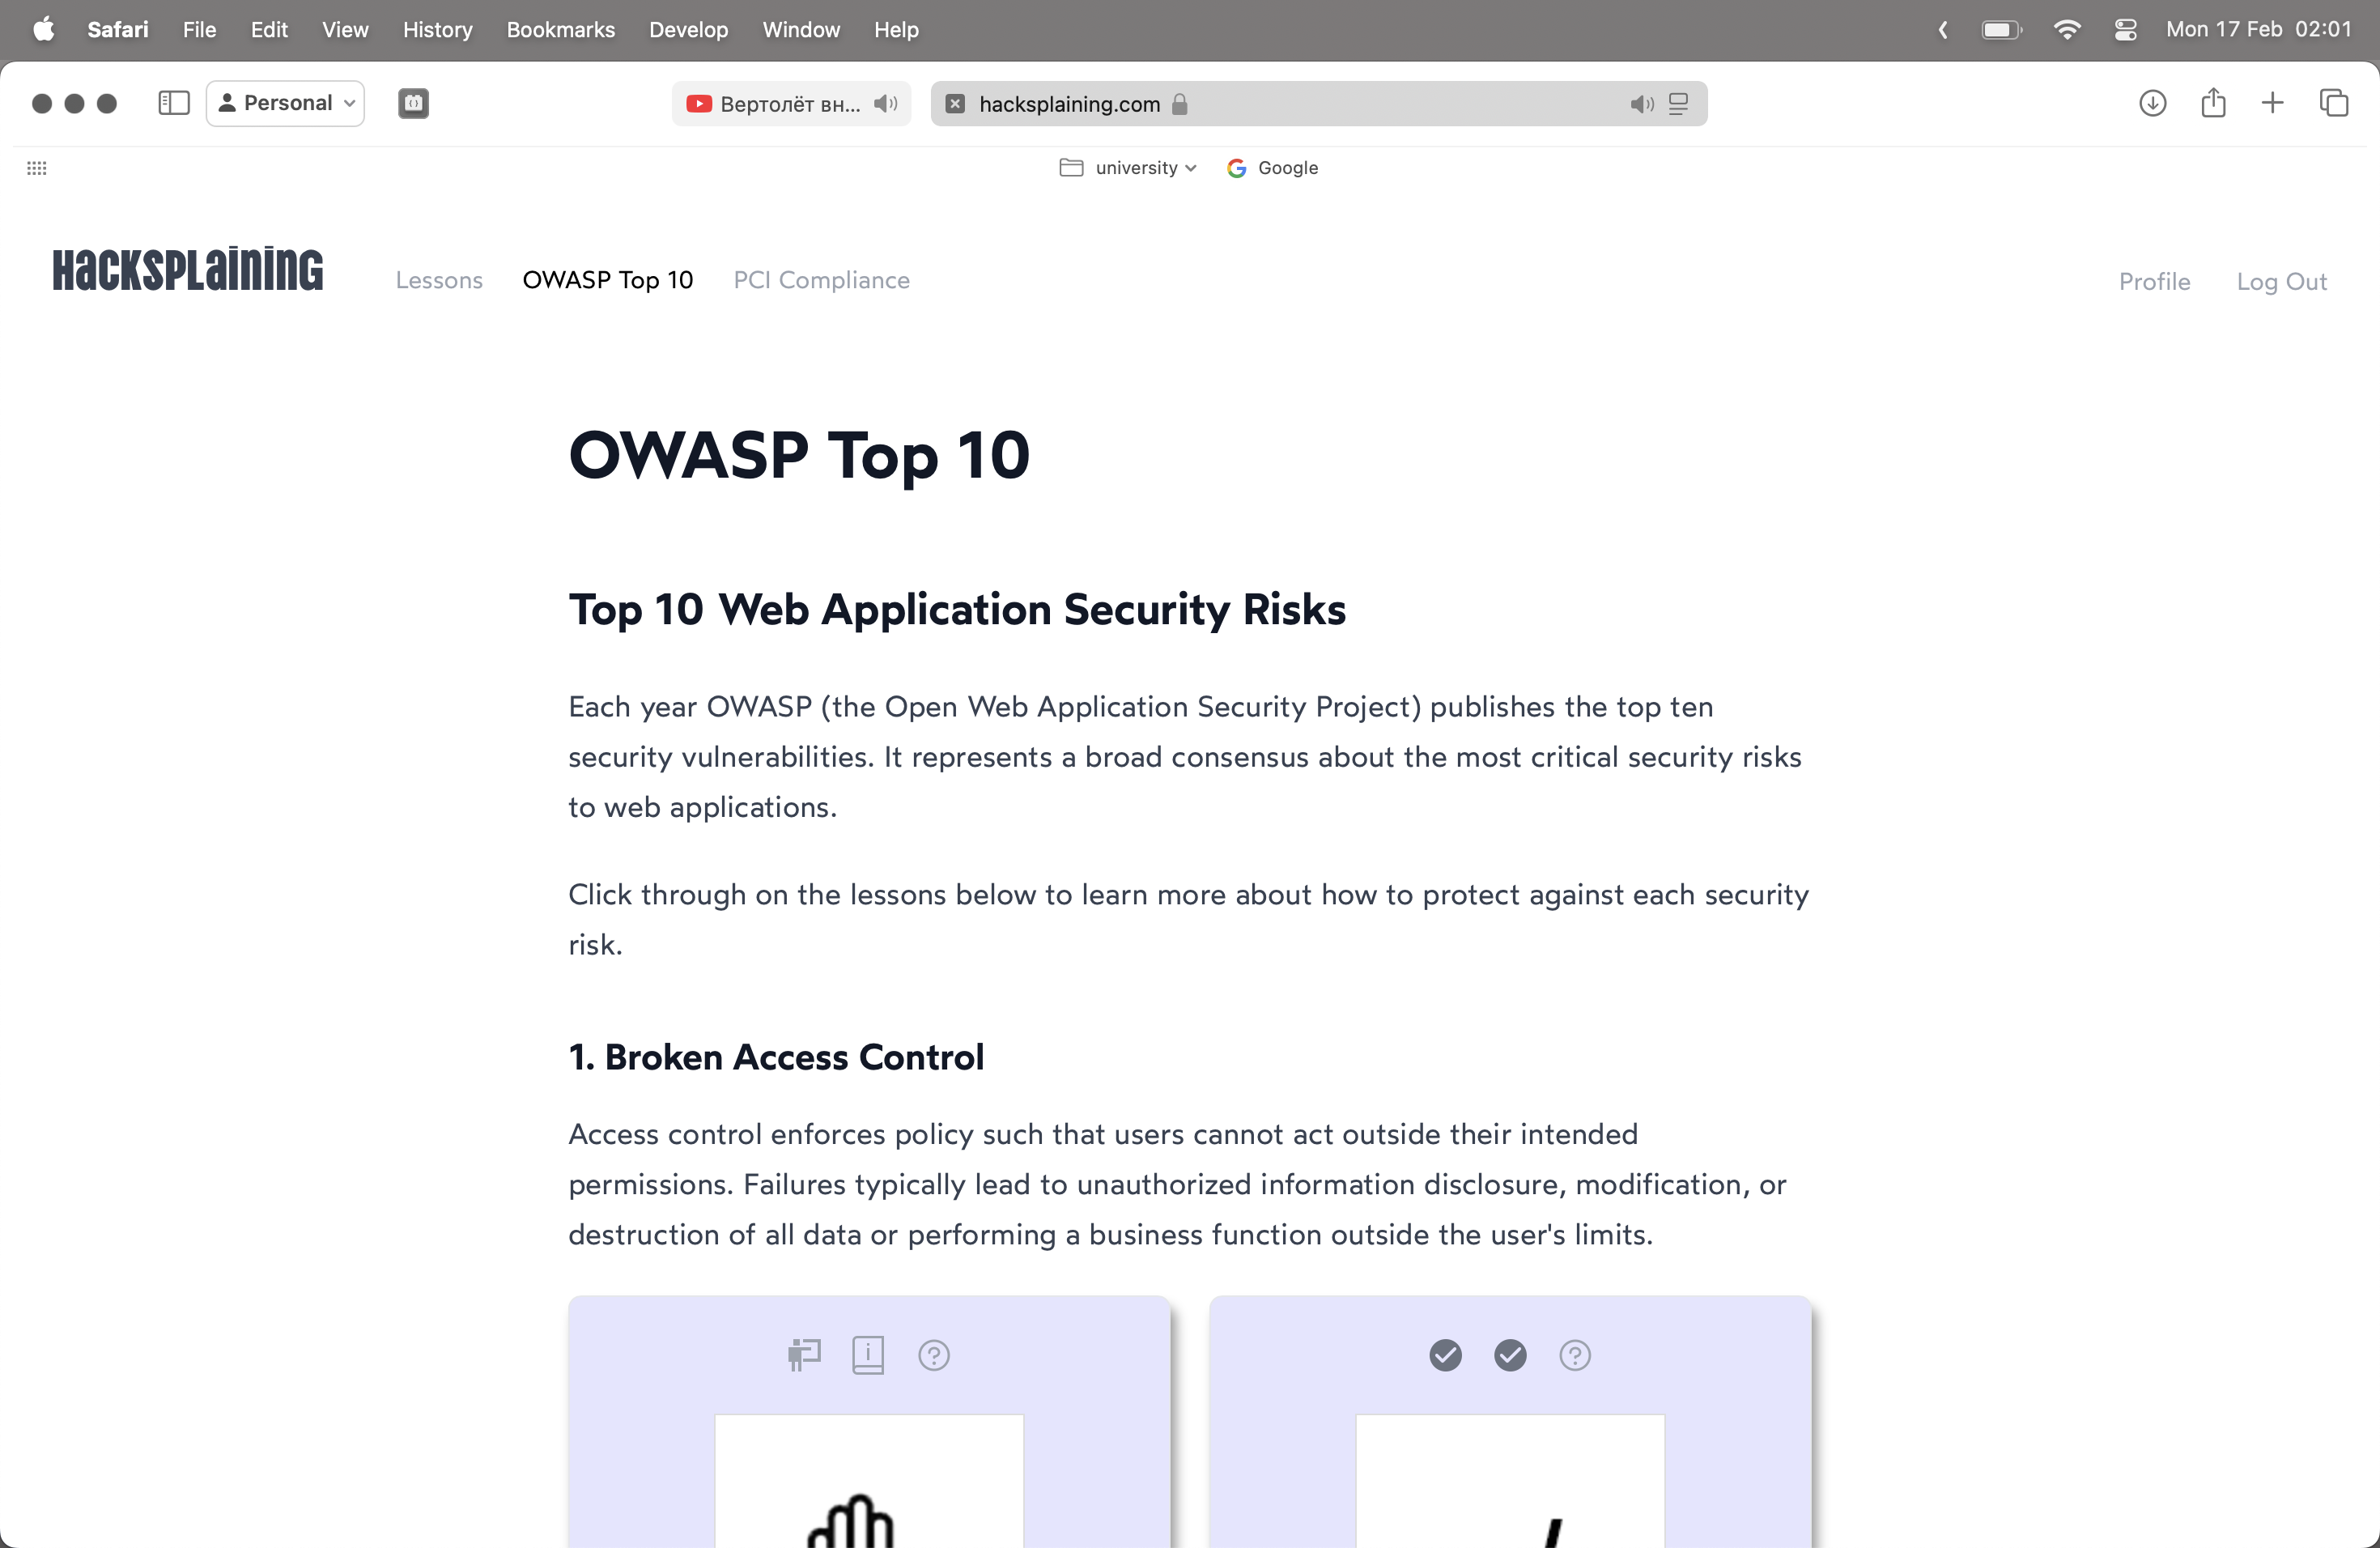
\includegraphics[width=1\textwidth]{Image5.png}

\subsection{Explore What OWASP Is}

OWASP stands for Open Web Application Security Project, a nonprofit foundation that works to improve the security of software. It provides open-source projects, tools, and methodologies for securing applications. The OWASP Top 10 is a standard awareness document that highlights the most critical security risks to web applications. 

\newpage

\subsubsection{Broken Access Control}
Access control ensures users act within their permissions. Failures can lead to unauthorized data access, modification, or destruction. \\
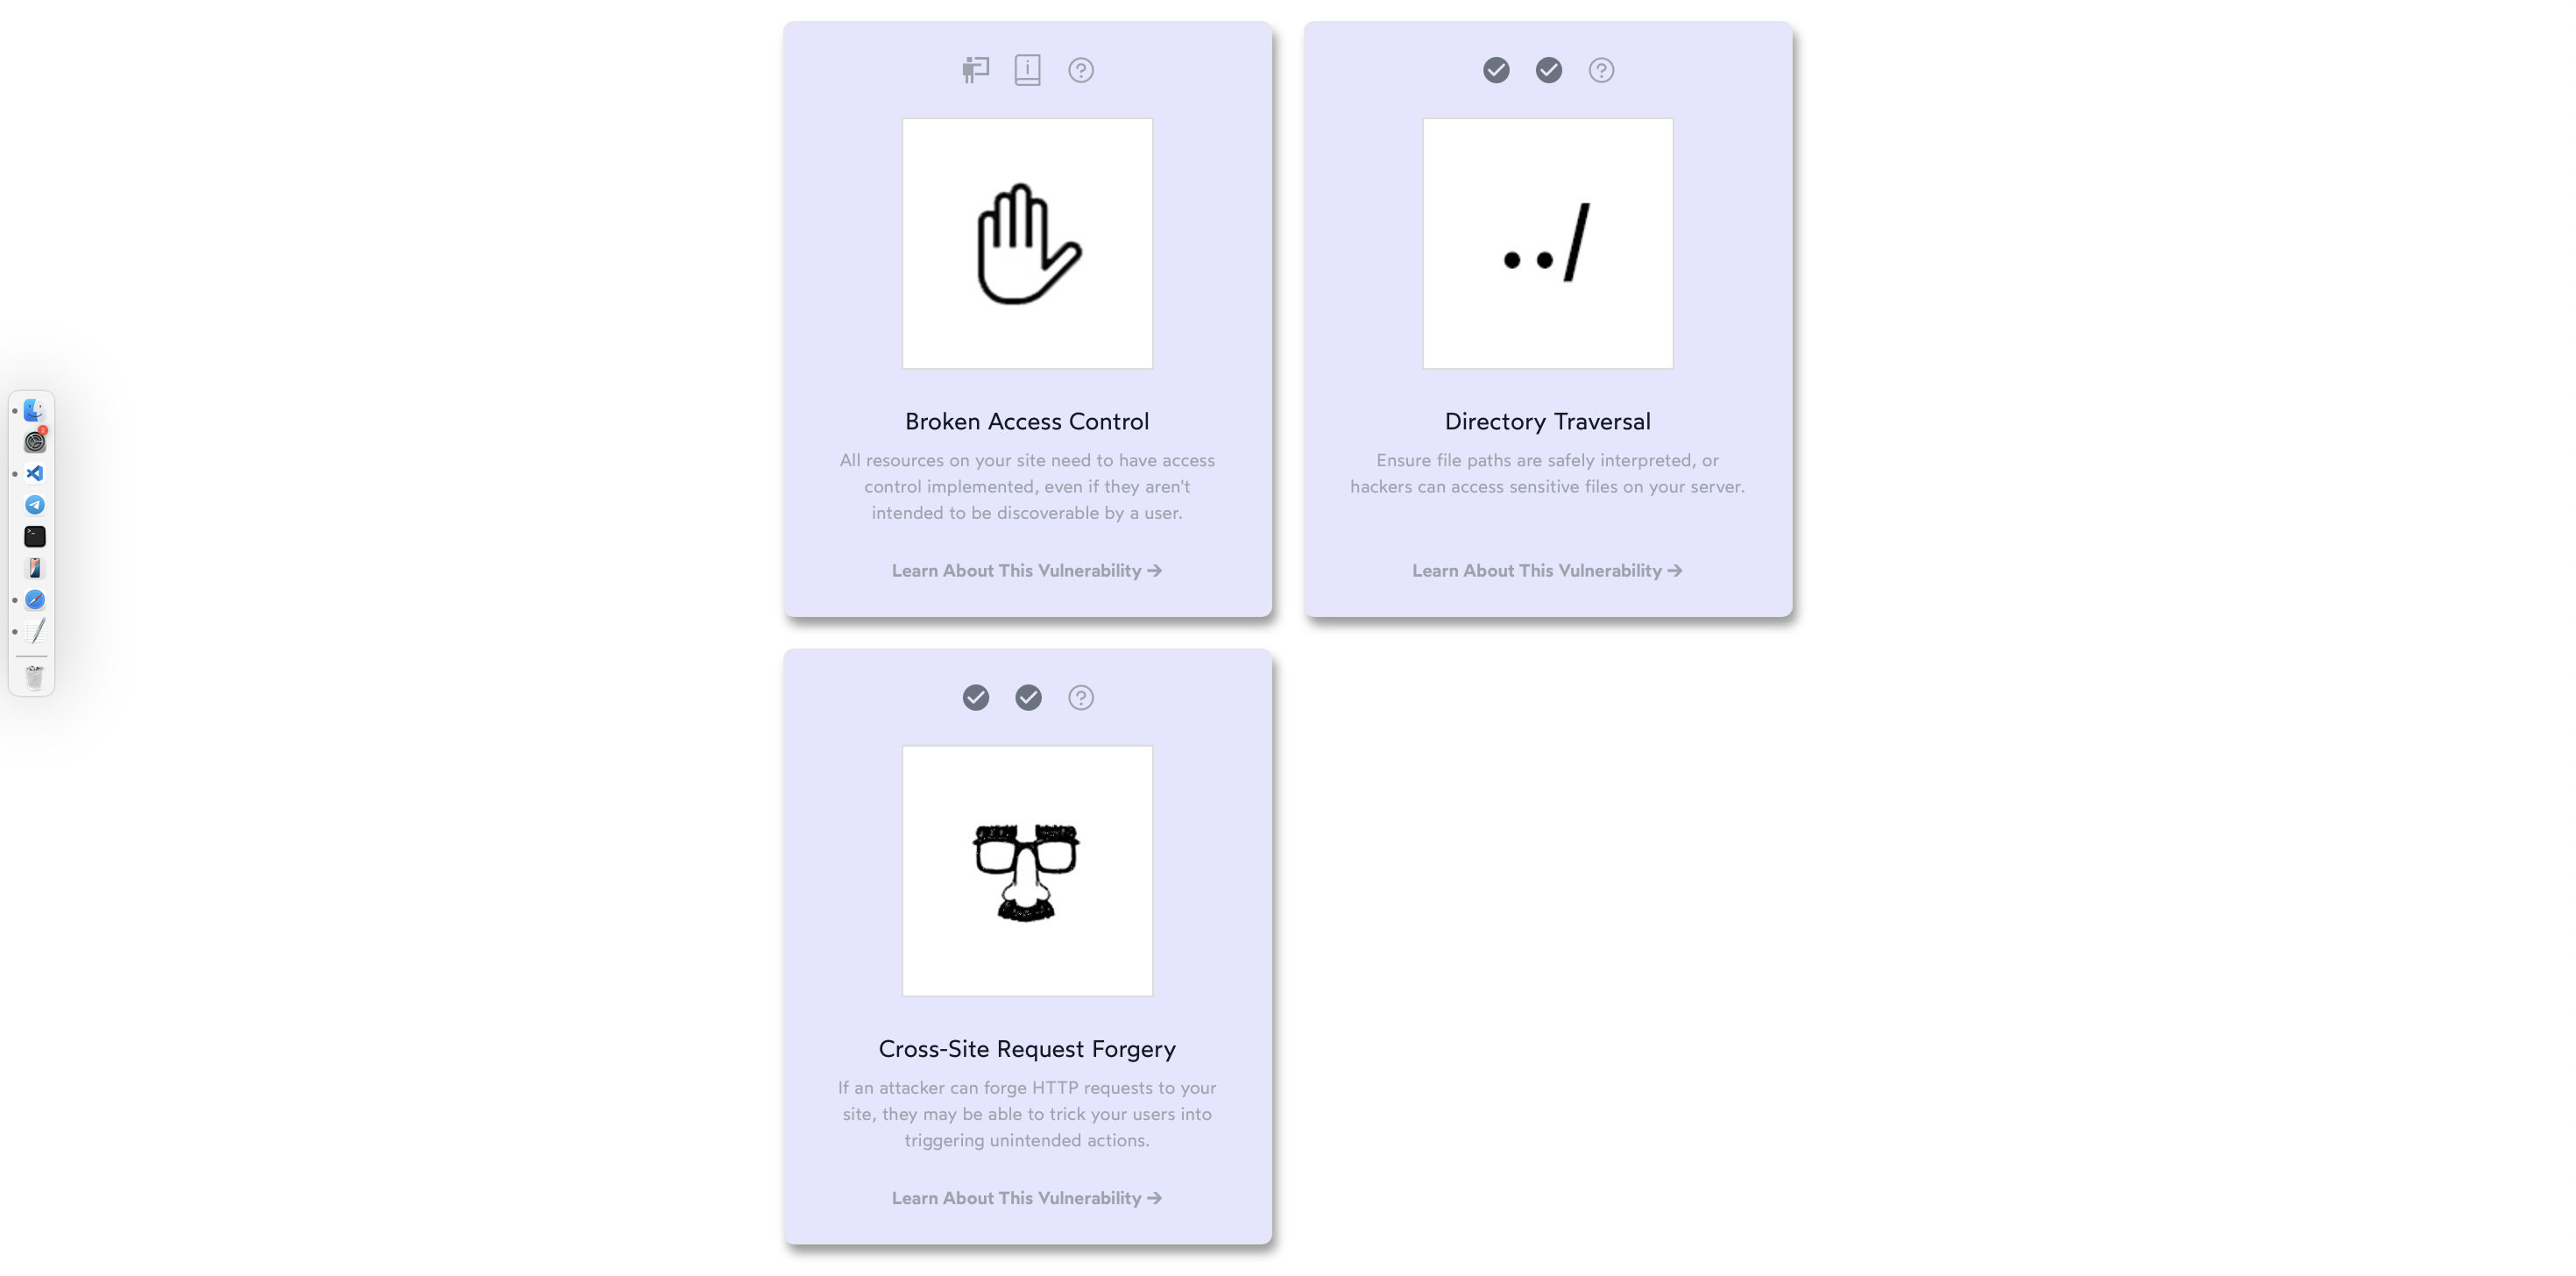
\includegraphics[width=1\textwidth]{Image6.png}

\subsubsection{Cryptographic Failures}
Cryptographic failures occur when sensitive data is not properly protected with strong encryption. This can lead to data theft, fraud, and other crimes. Protection methods include encrypting data at rest and in transit using modern encryption algorithms.
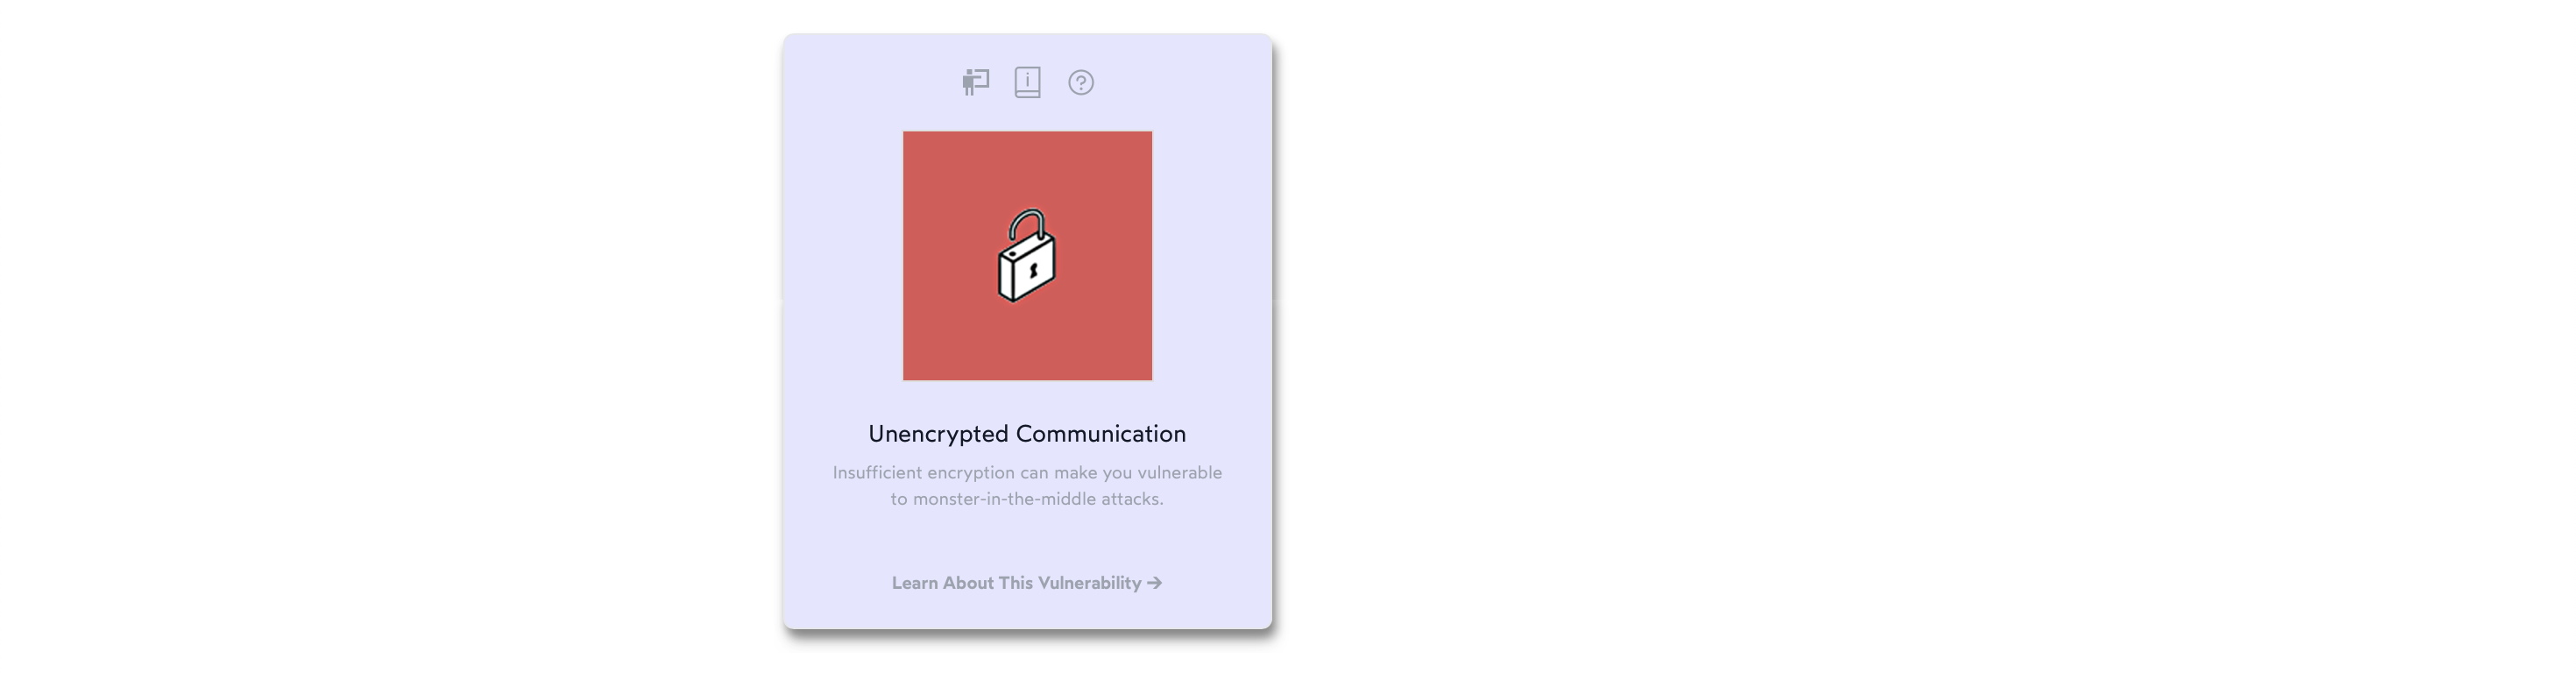
\includegraphics[width=1\textwidth]{Image7.png}

\subsubsection{Injection}
Injection flaws, such as SQL, NoSQL, OS, and LDAP injection, occur when untrusted data is sent to an interpreter as part of a command or query. This can lead to unauthorized data access or execution of unintended commands. Protection methods include using parameterized queries and input validation. \\
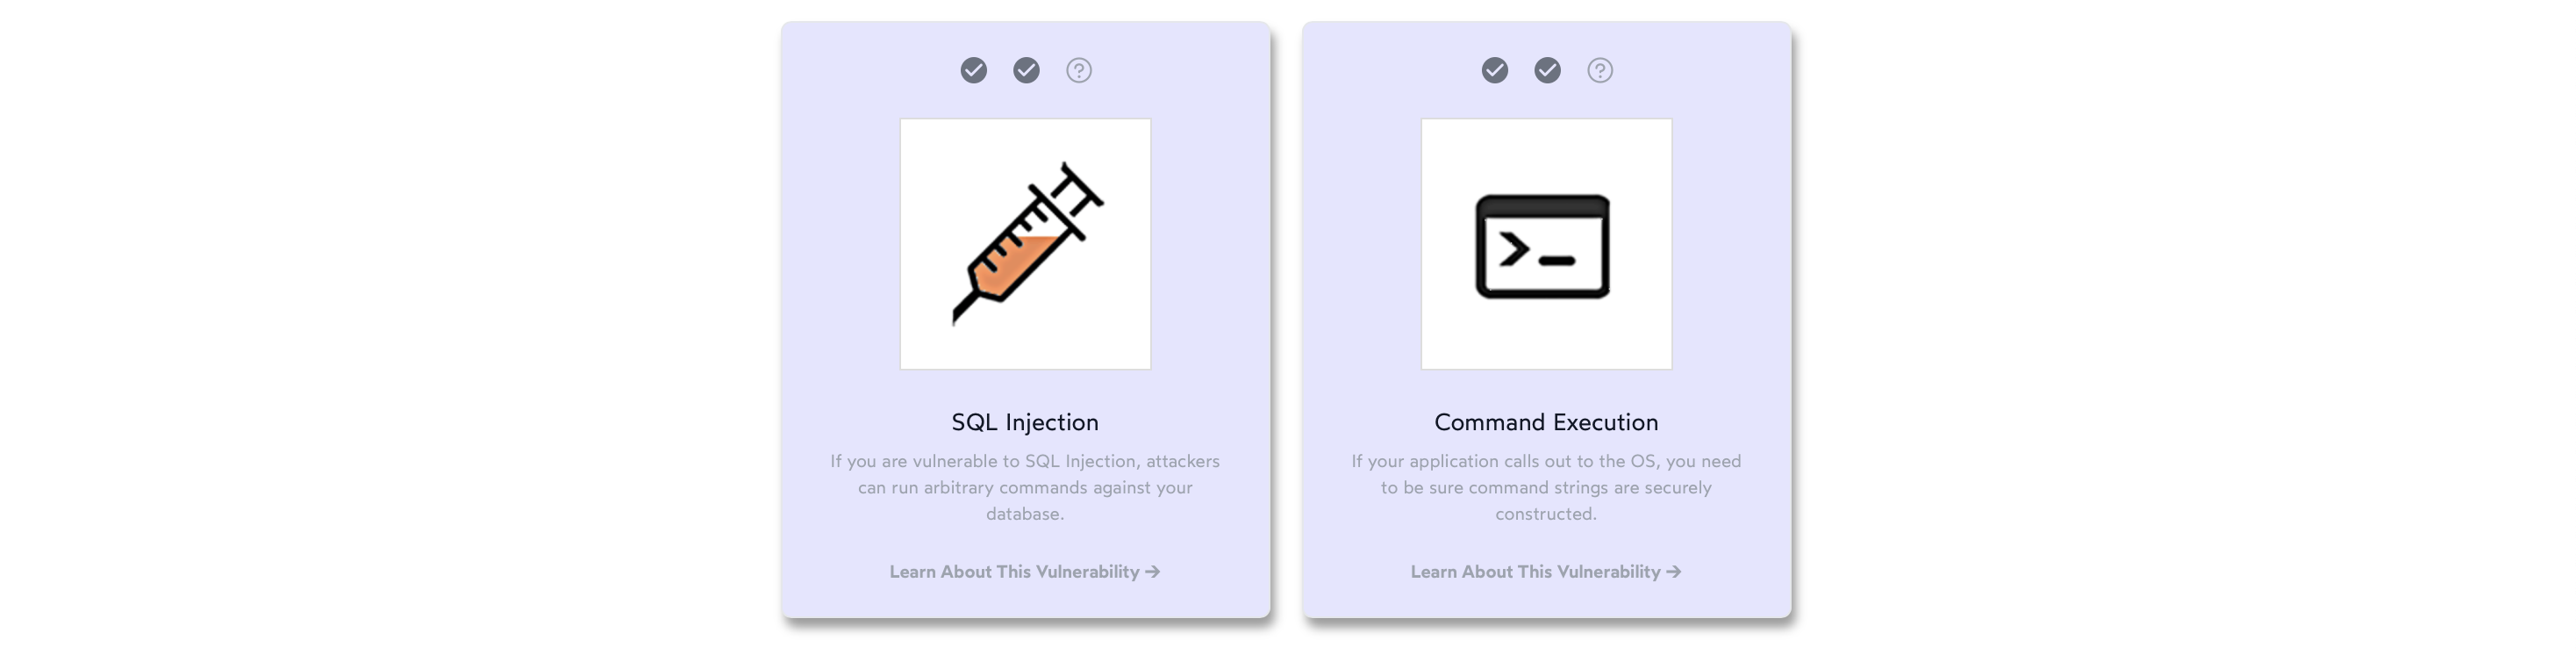
\includegraphics[width=1\textwidth]{Image8.png}

\subsubsection{Insecure Design}
Insecure design refers to the lack of security considerations during the design phase of software development. This can lead to vulnerabilities that are difficult to fix later. Protection methods include gathering security requirements, threat modeling, and regular security testing. \\
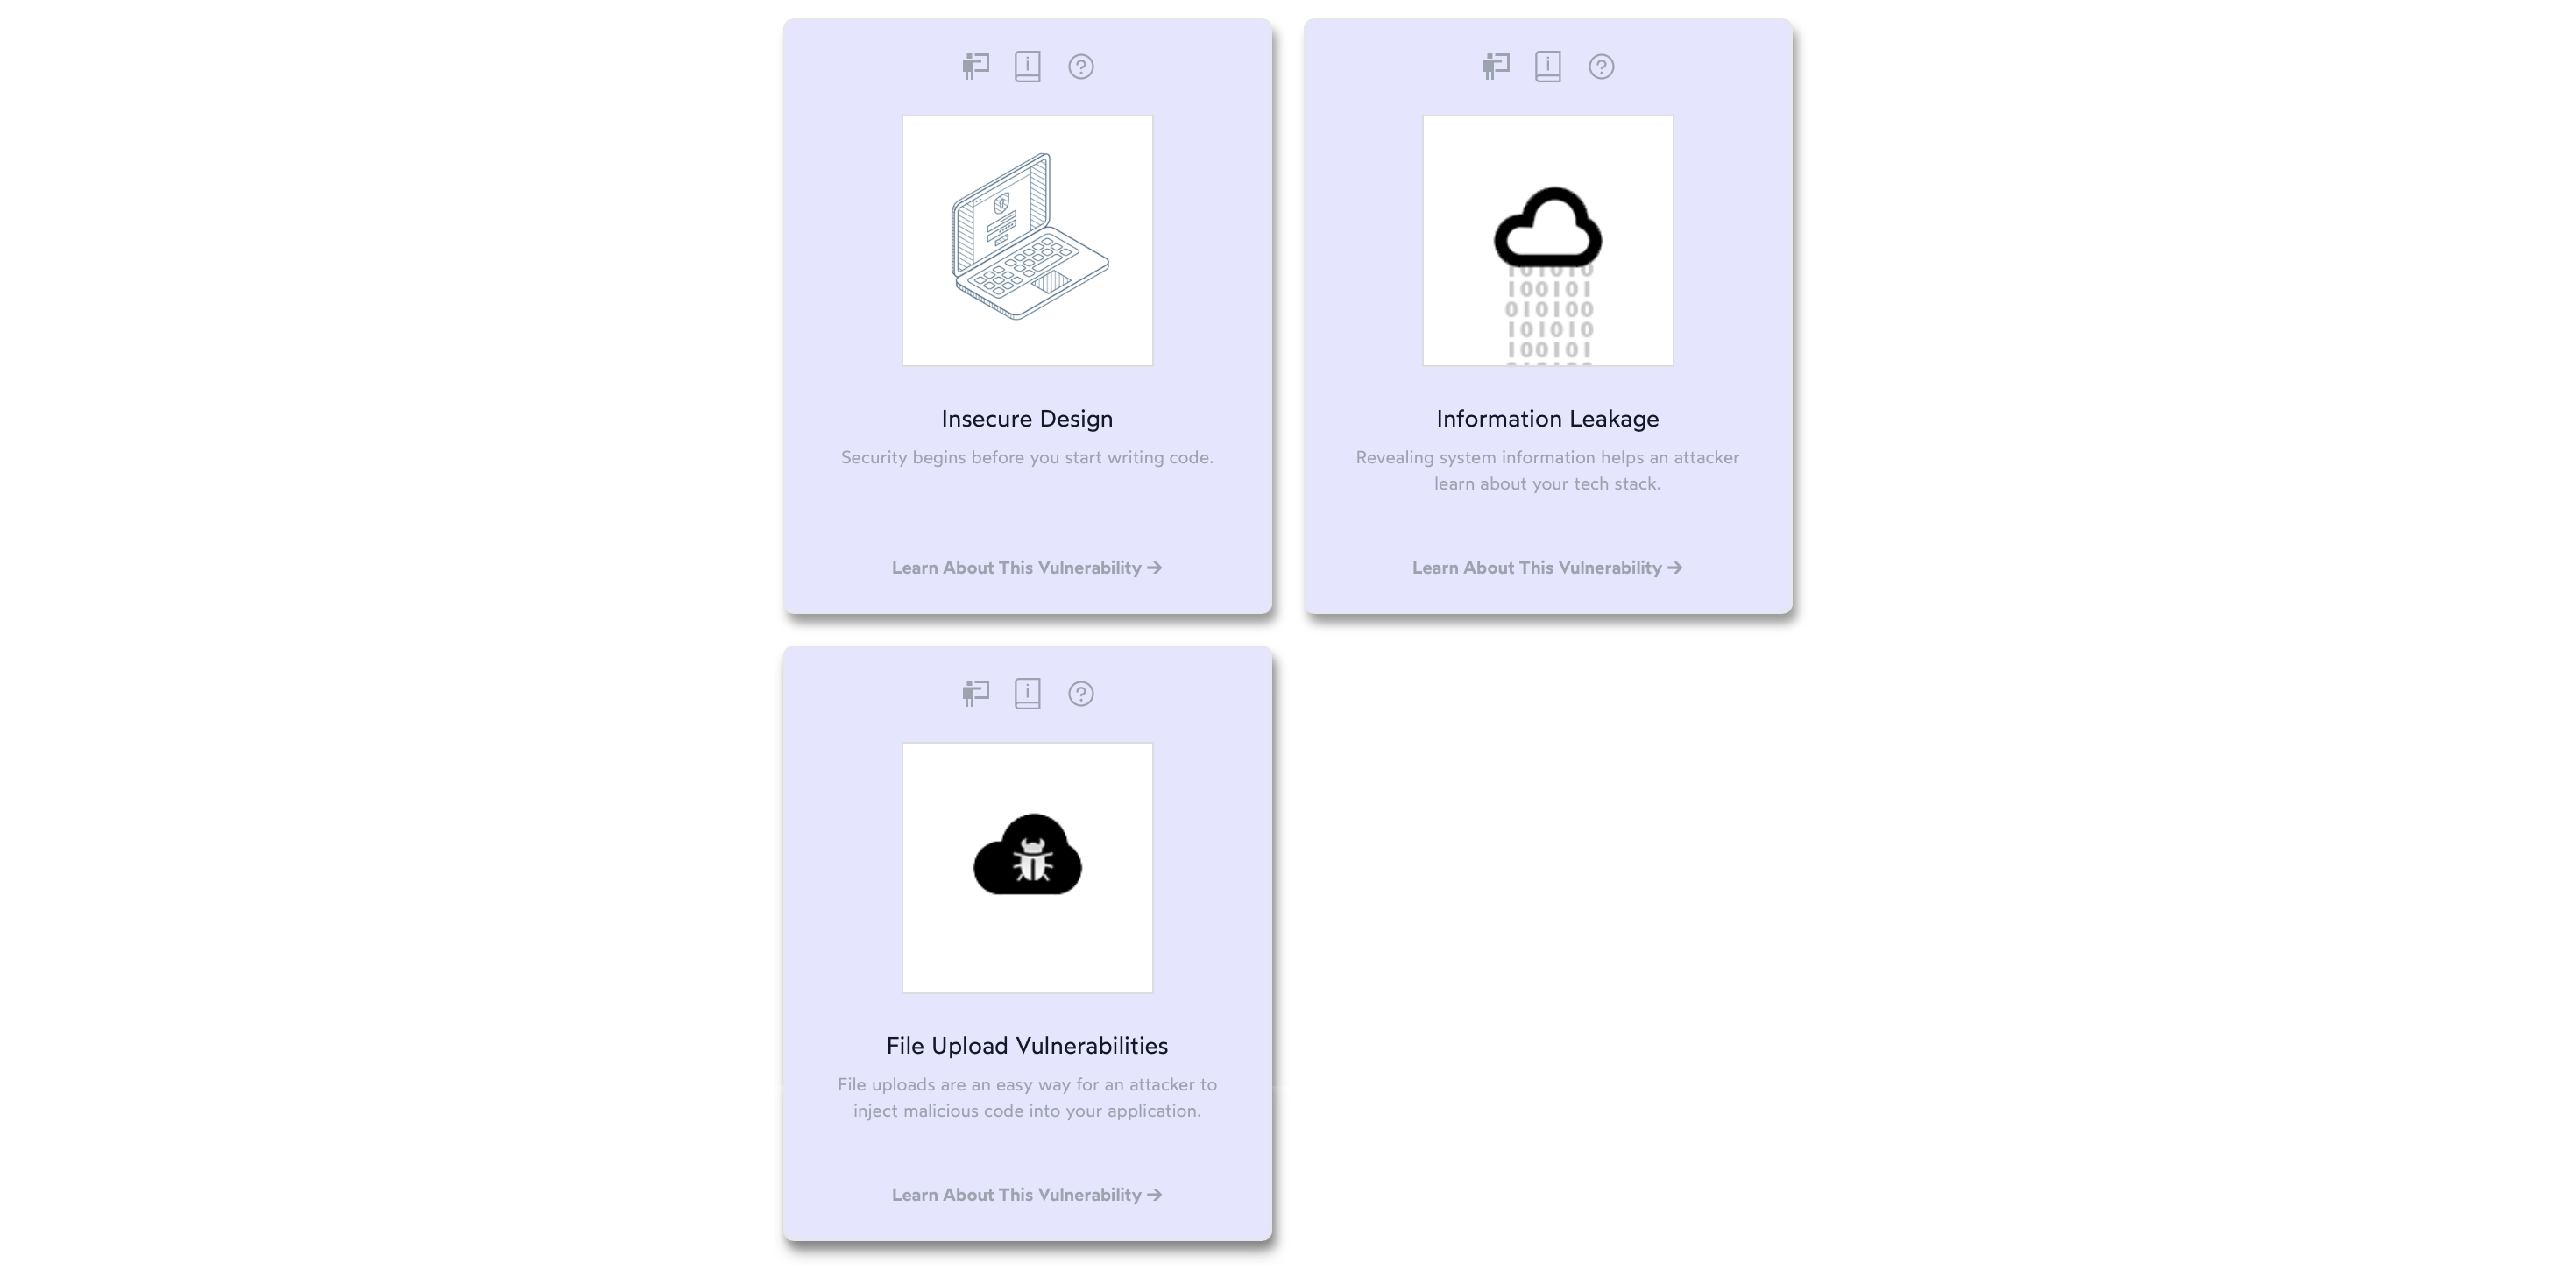
\includegraphics[width=1\textwidth]{Image9.png}

\subsubsection{Security Misconfiguration}
Security misconfiguration occurs when software is not securely configured, leading to vulnerabilities such as default accounts, open cloud storage, and verbose error messages. Protection methods include secure configuration standards, regular patching, and timely upgrades. \\
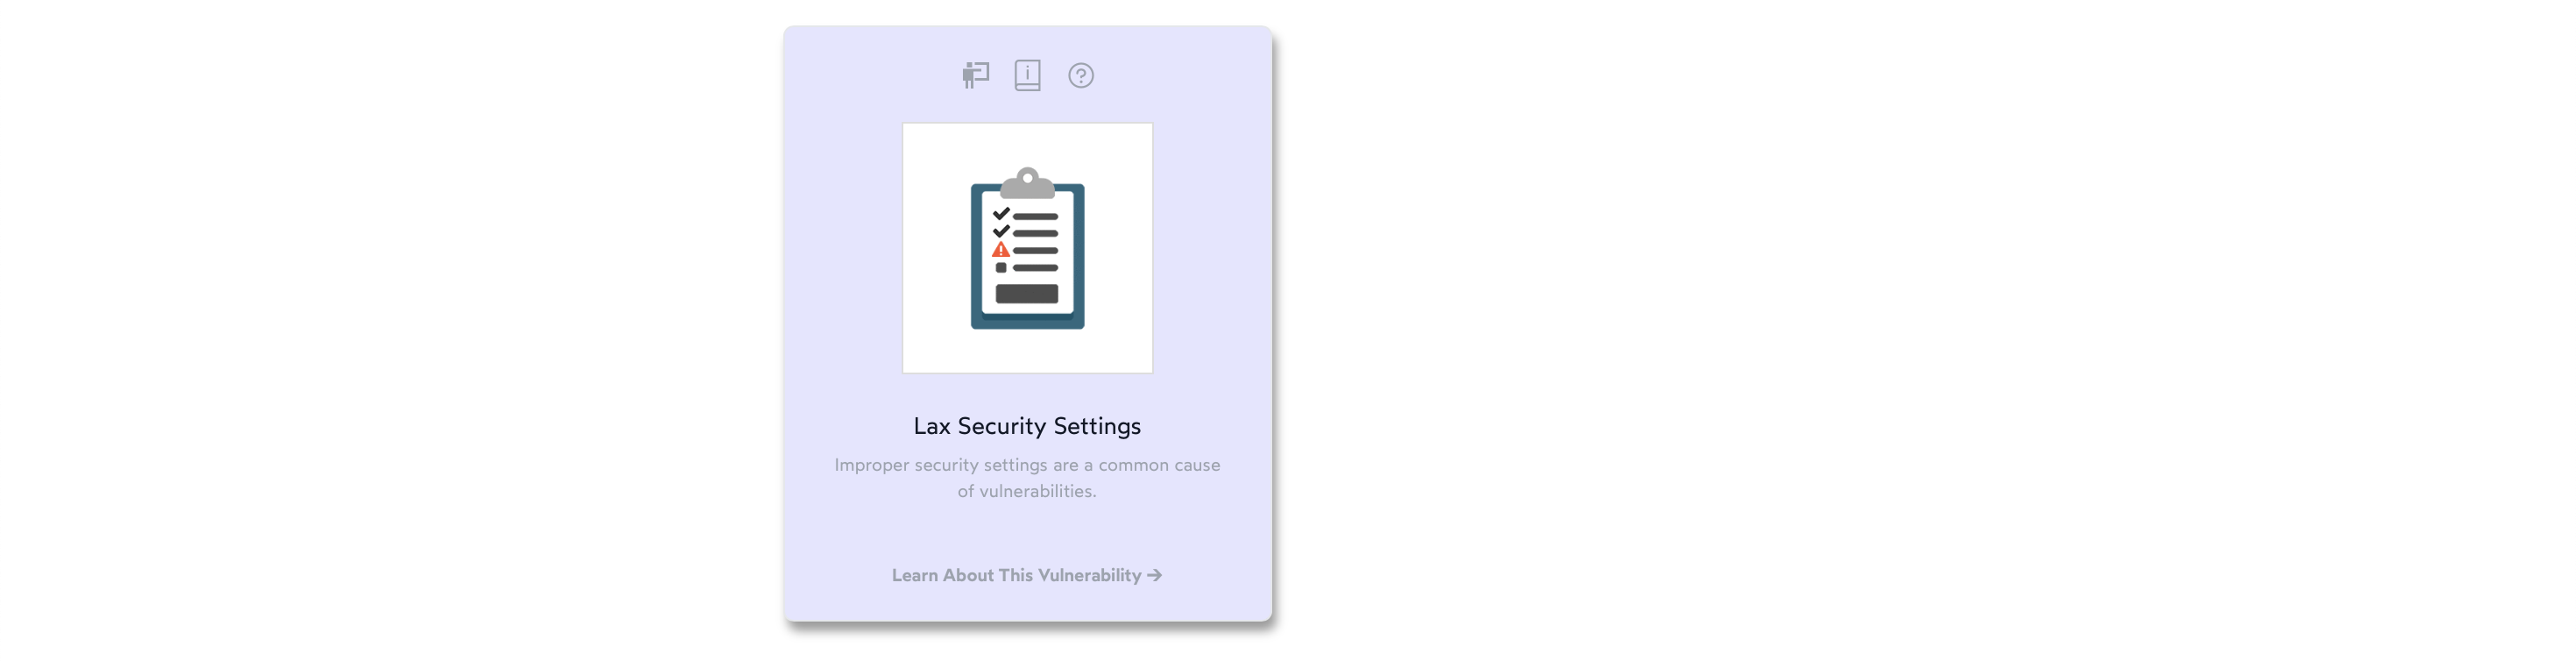
\includegraphics[width=1\textwidth]{Image10.png}

\newpage

\subsubsection{Vulnerable and Outdated Components}
Using vulnerable or outdated components, such as libraries and frameworks, can introduce security risks. Protection methods include regularly updating components and using tools to identify known vulnerabilities. \\ 
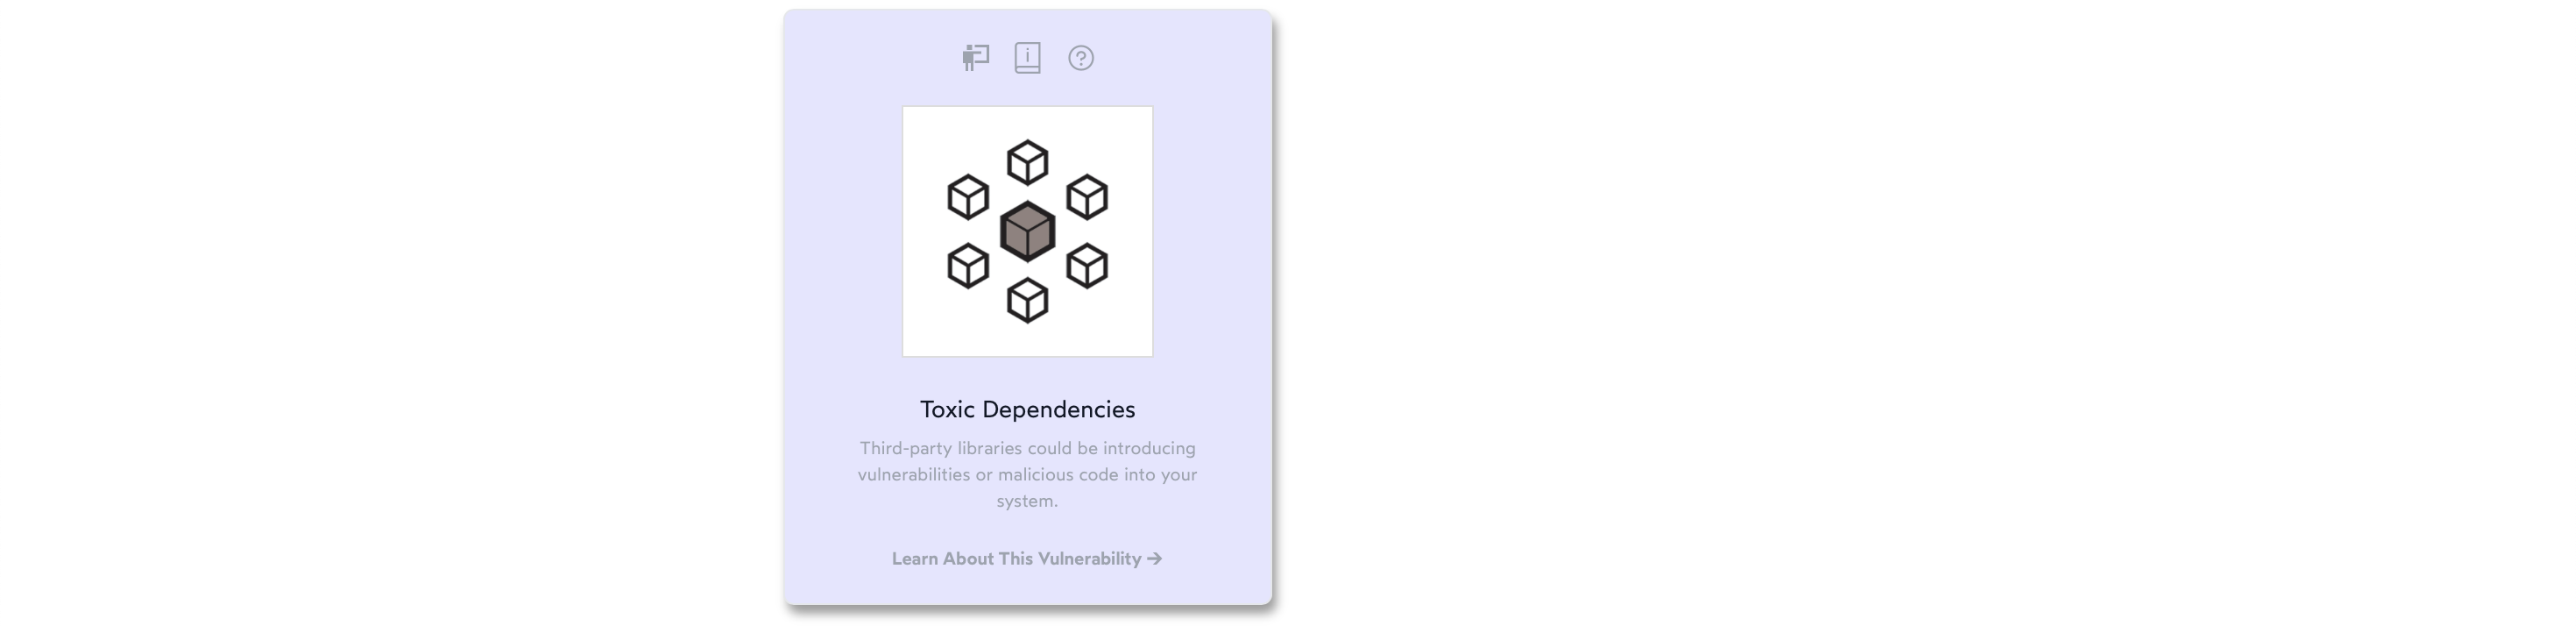
\includegraphics[width=1\textwidth]{Image11.png}

\subsubsection{Identification and Authentication Failures}
Failures in identification and authentication can lead to compromised passwords, session tokens, and user identities. Protection methods include strong password policies, multi-factor authentication, and secure session management. \\
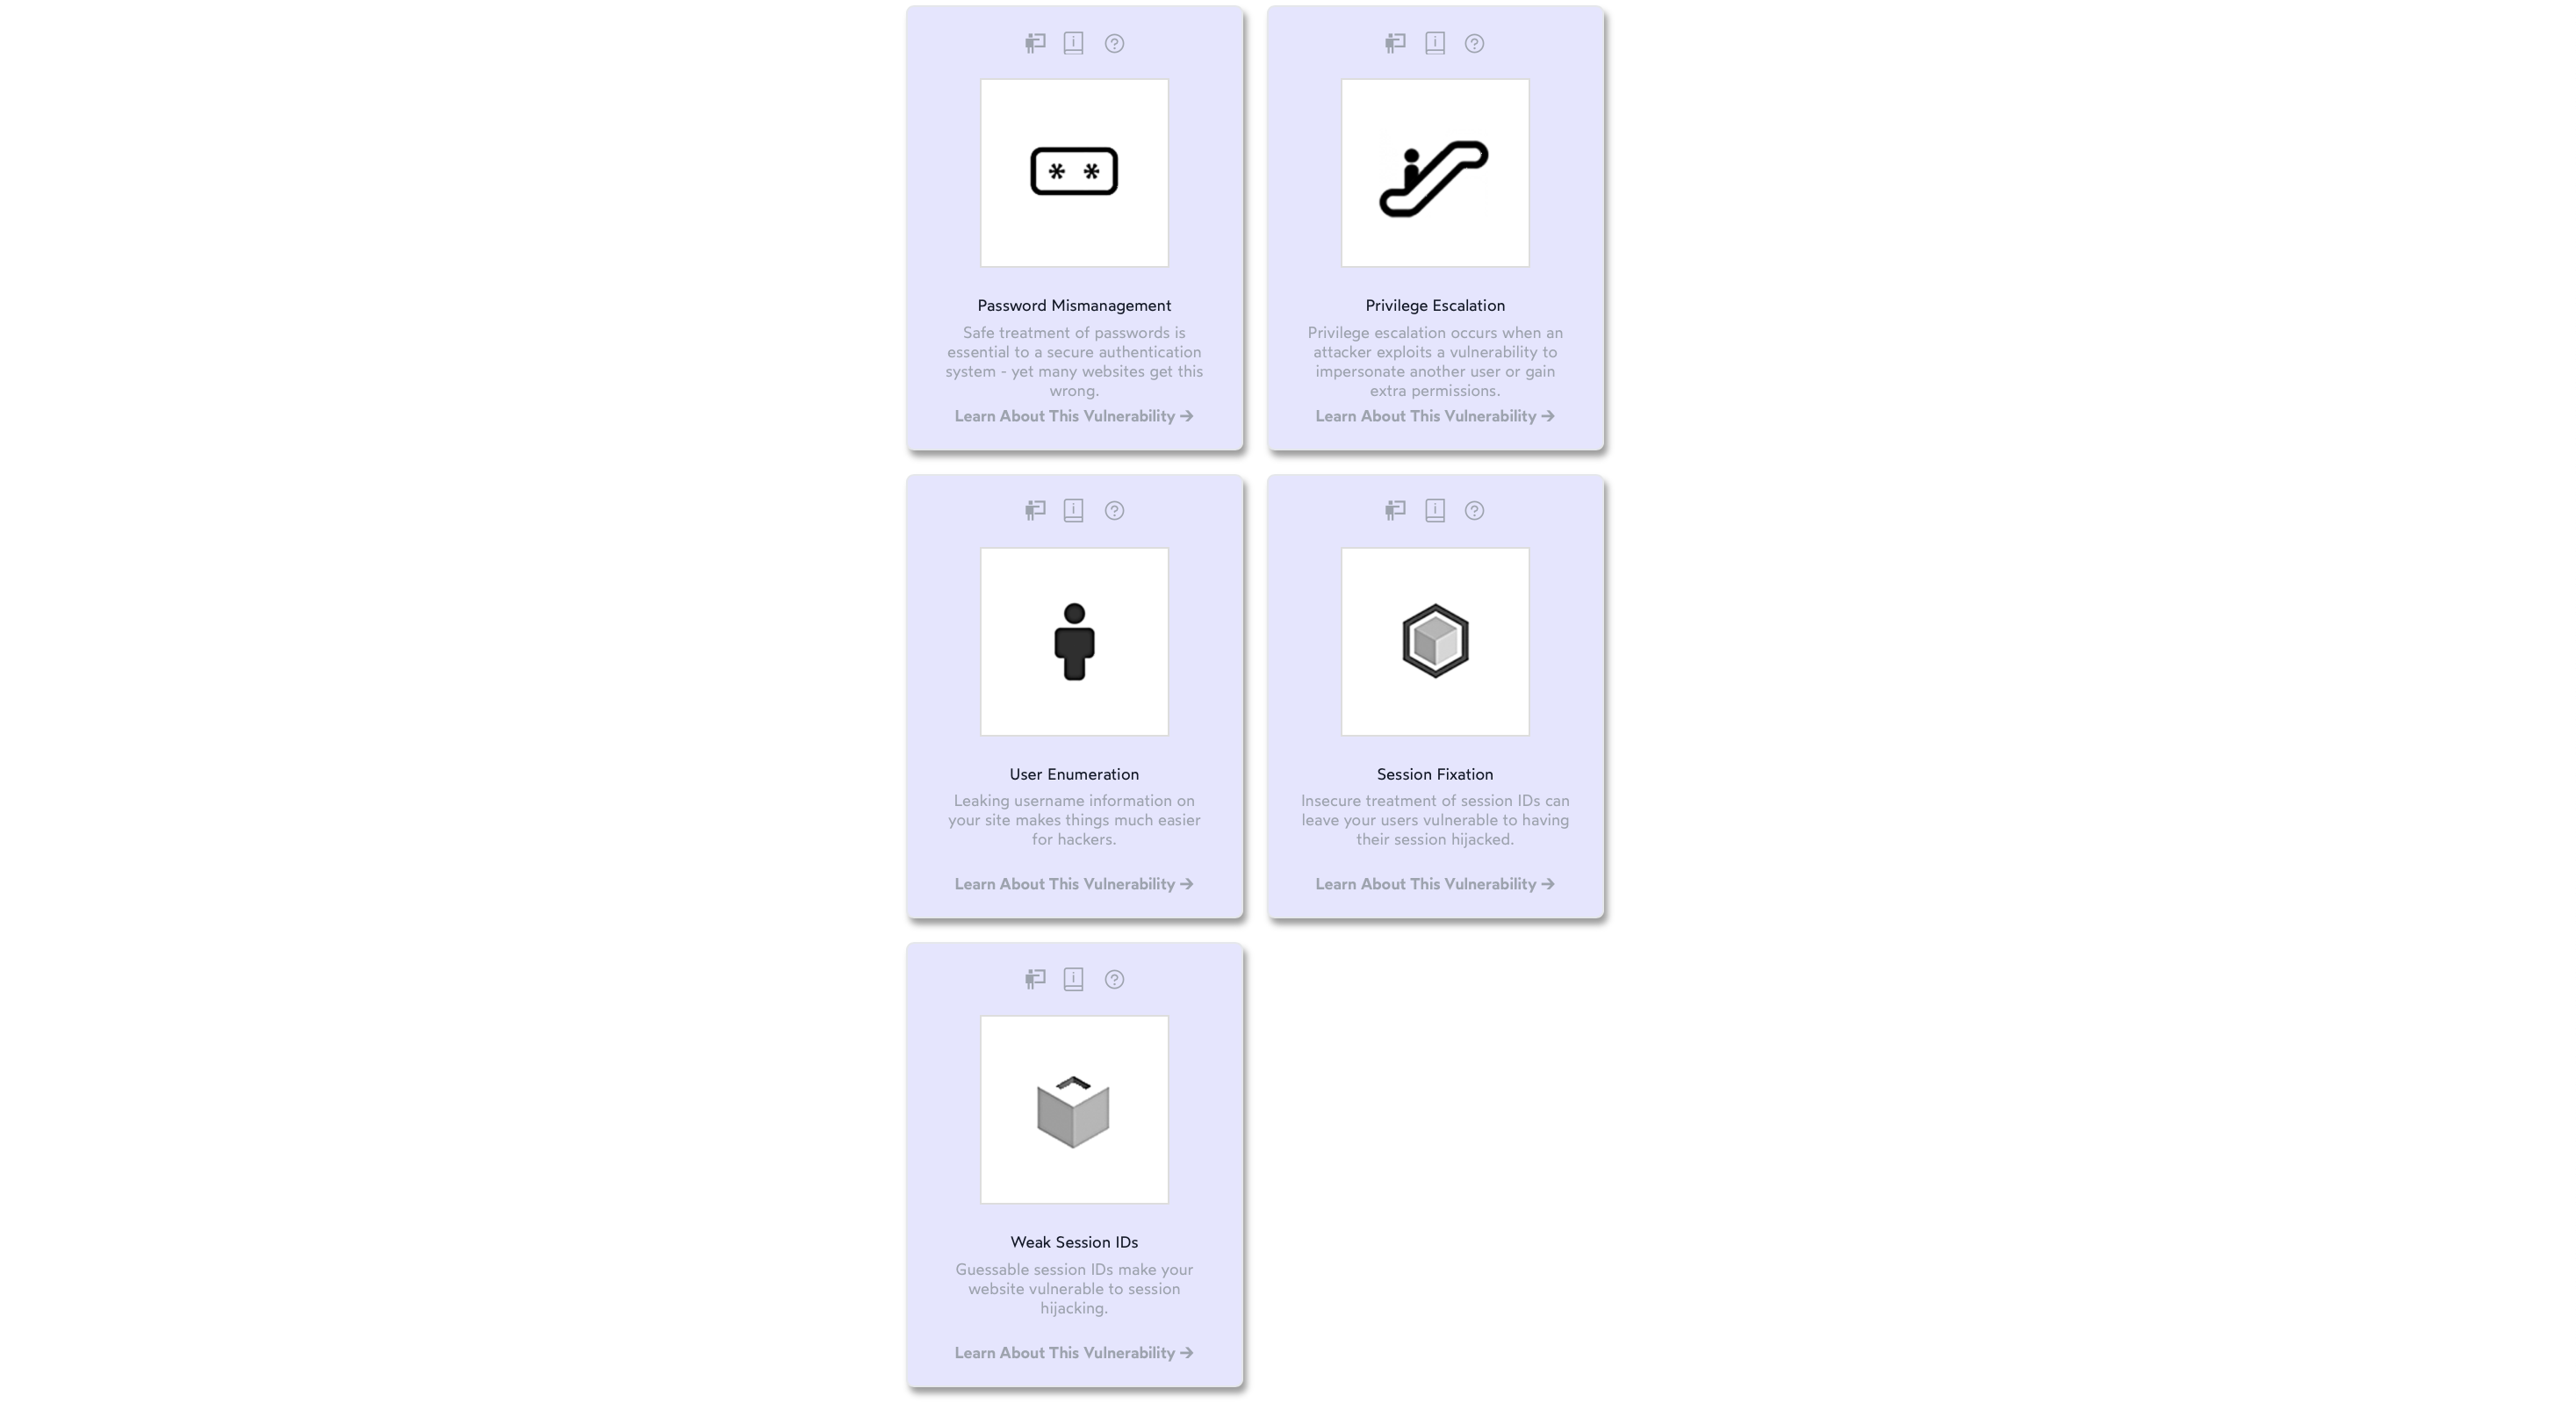
\includegraphics[width=1\textwidth]{Image12.png}

\subsubsection{Software and Data Integrity Failures}
Software and data integrity failures occur when code and infrastructure do not protect against integrity violations. This can lead to unauthorized access and malicious code execution. Protection methods include using trusted sources, verifying updates, and securing the deployment pipeline.

\newpage

\subsubsection{Security Logging and Monitoring Failures}
Insufficient logging and monitoring can allow attackers to go undetected for long periods. Protection methods include comprehensive logging, real-time monitoring, and effective incident response integration. \\
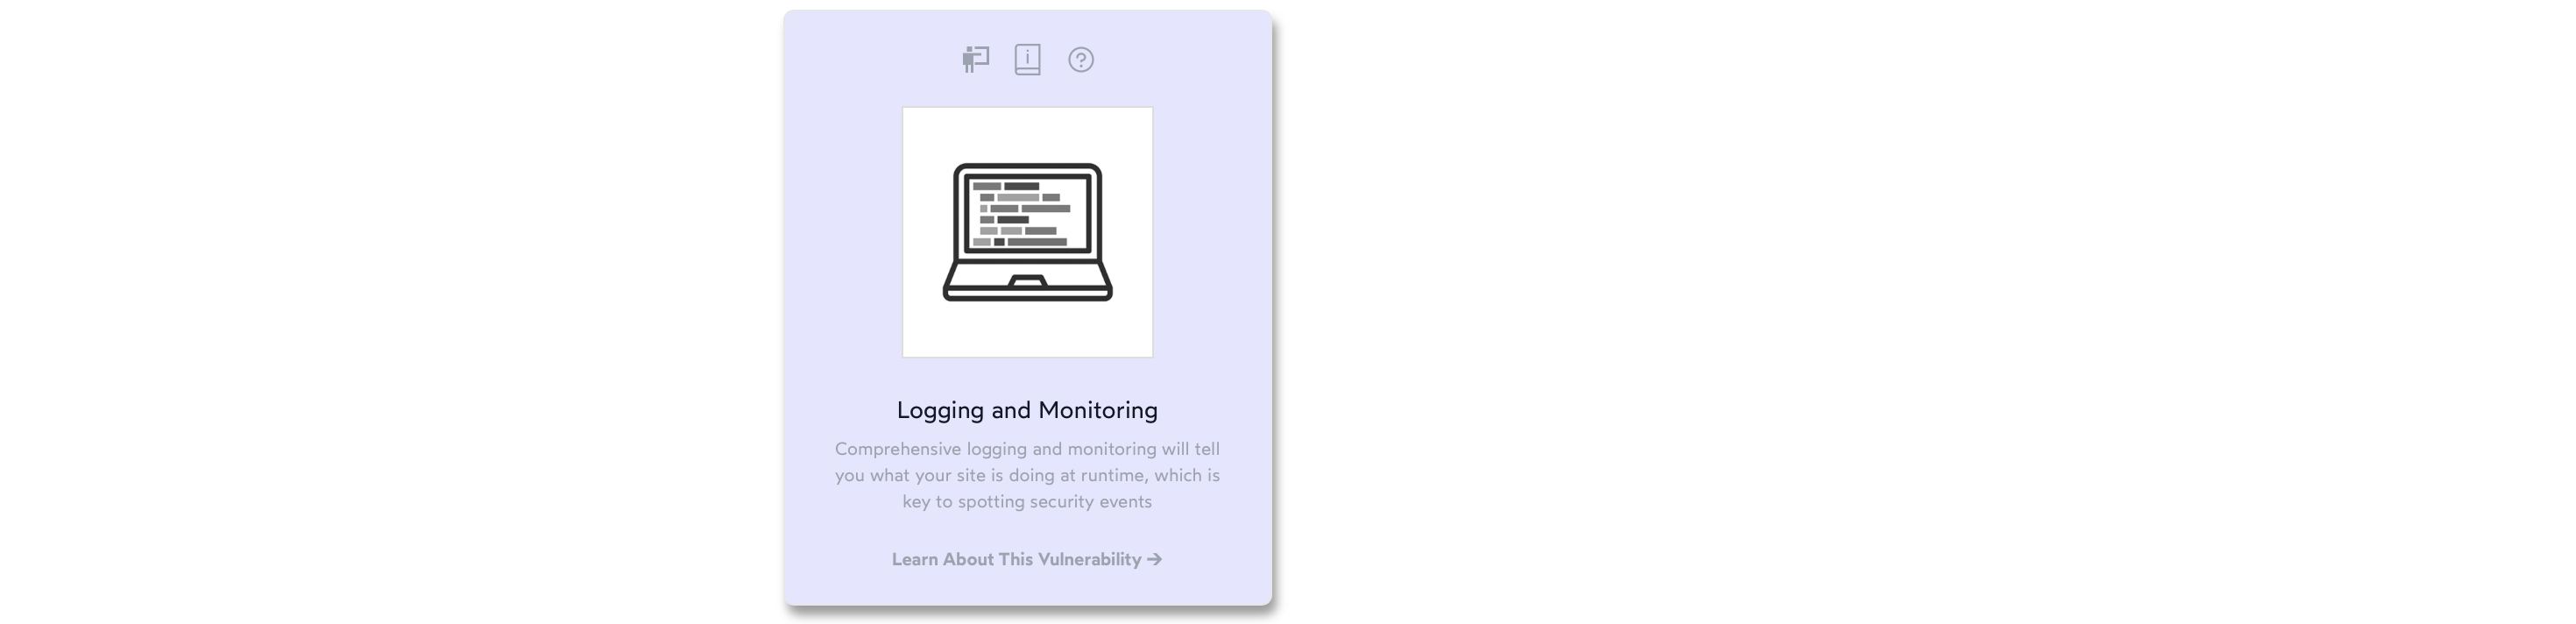
\includegraphics[width=1\textwidth]{Image13.png}

\subsubsection{Server-Side Request Forgery}
Server-Side Request Forgery (SSRF) occurs when a web application fetches a remote resource without validating the user-supplied URL. This can lead to unauthorized requests to internal systems. Protection methods include validating and sanitizing URLs and implementing network access controls. \\
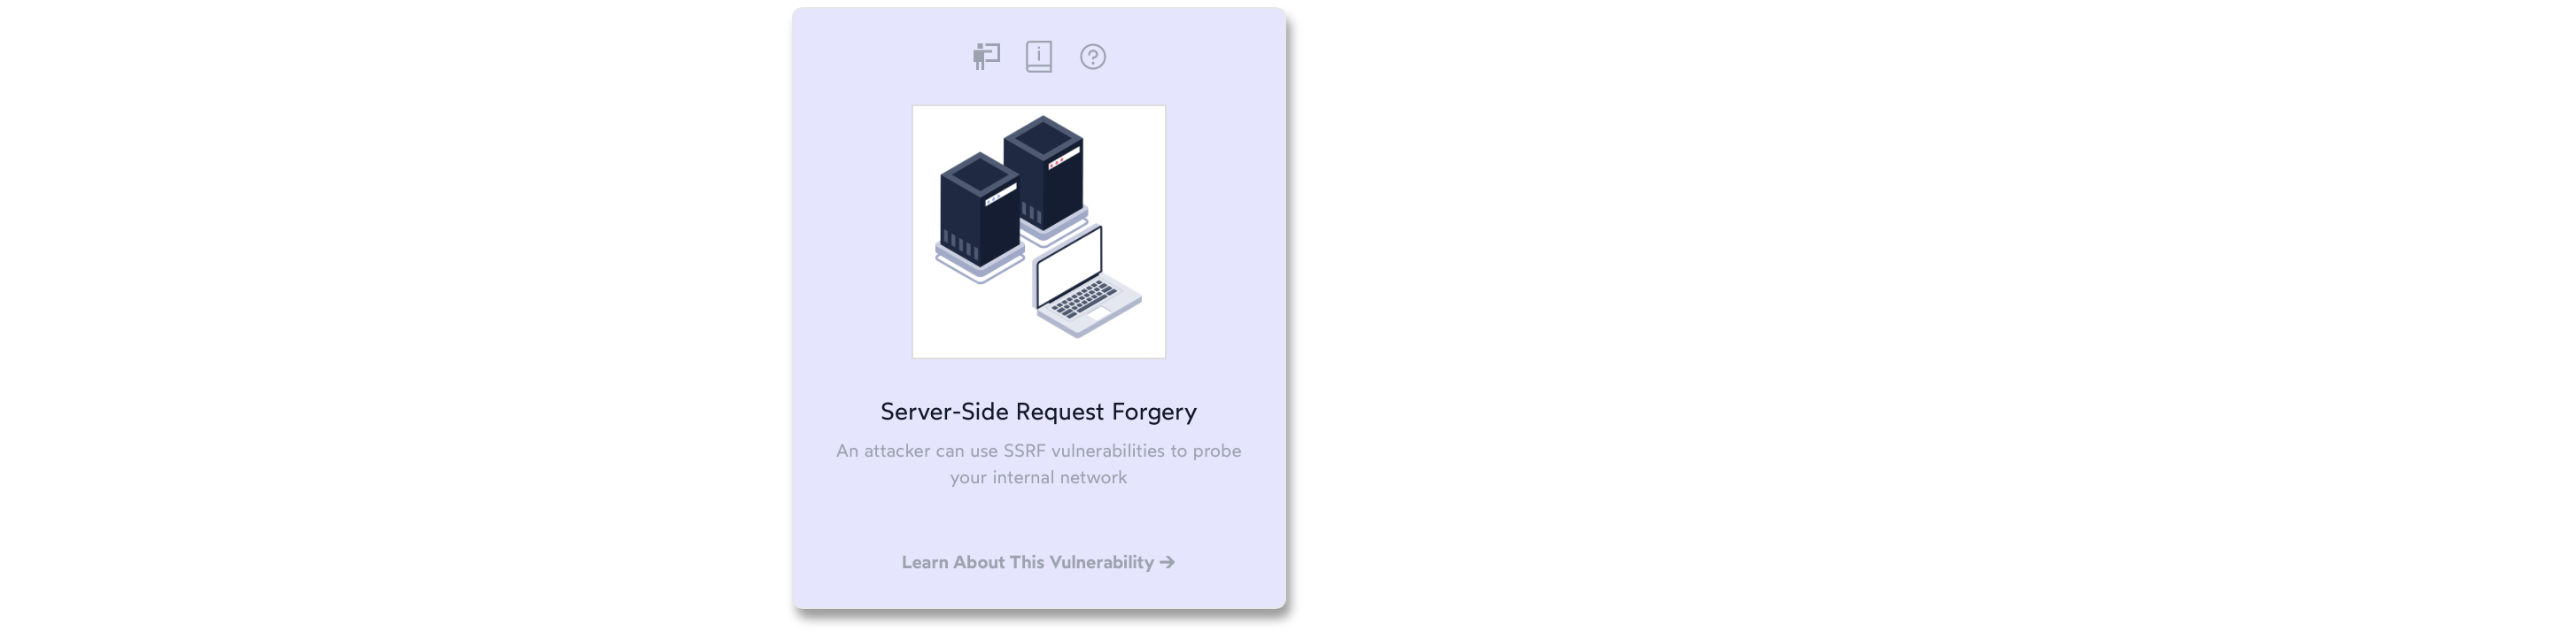
\includegraphics[width=1\textwidth]{Image14.png}

\section{Lab Completion}

In the end of Laboratory work, I have learned about the most common web application vulnerabilities and how to protect against them. I have explored the Hacksplaining Security Training for Developers and the OWASP Top 10 web application security risks. I have gained valuable insights into the importance of secure coding practices and the need for continuous security awareness.

\end{document}